\documentclass[UTF8,twoside]{ctexrep}

% === BEGIN INLINE: template/template/preamble.tex ===
\usepackage{url}
\usepackage{gbt7714}
\usepackage{geometry}
\usepackage{fancyhdr}
\usepackage{setspace}
\usepackage{booktabs}
\usepackage{multirow}
\usepackage{amssymb,amsmath}
\usepackage{graphicx}
\graphicspath{{../../../}{../../templates/CDU_thesis_latex/}{../}{./}}
\usepackage{subcaption}
\usepackage{float}
\usepackage{enumitem}
\usepackage{etoolbox}
\usepackage{xeCJK}
\usepackage{fontspec}
\usepackage{array}
\usepackage{algorithm}
\usepackage{algorithmicx}
\usepackage{algpseudocode}
\usepackage{pifont}

% 全局西文字体：正文中的英文和阿拉伯数字默认使用 Times New Roman。
\setmainfont{Times New Roman}

\bibliographystyle{gbt7714-numerical}
\makeatletter
\def\NAT@cmprs{\@ne}
\patchcmd{\NAT@citexnum}
  {\def@NAT@last@yr{-\NAT@penalty}}
  {%
    \ifx\NAT@last@yr\relax
      \def@NAT@last@yr{\@citea}%
    \else
      \def@NAT@last@yr{-\NAT@penalty}%
    \fi
  }
  {}{\PackageWarning{thesis}{Failed to patch citation compression}}
\makeatother

\newcommand{\TNR}[1]{{\rmfamily #1}}
\newcommand{\circnum}[1]{\ding{\numexpr171+#1\relax}}
% === END INLINE: template/template/preamble.tex ===
\usepackage{longtable}
\usepackage{float}
\usepackage{tikz}
\usetikzlibrary{shapes.geometric,arrows.meta,positioning,calc}

% === BEGIN INLINE: chapters/00_custom_macros.tex ===
\makeatletter
\newcommand{\YogaCaptionNoColon}[1]{%
  \begingroup
  \renewcommand{\@makecaption}[2]{%
    \vskip 6pt%
    \sbox\@tempboxa{\small ##1\quad ##2}%
    \ifdim \wd\@tempboxa >\hsize
      {\small ##1\quad ##2\par}%
    \else
      \global\@minipagefalse
      \hb@xt@\hsize{\hfil\box\@tempboxa\hfil}%
    \fi
    \vskip\belowcaptionskip}%
  \caption{#1}%
  \endgroup}
\makeatother

\newcommand{\YogaSystemArchitectureTikZ}{%
\resizebox{\textwidth}{!}{%
\begin{tikzpicture}[
  node distance=0.9cm and 0.8cm,
  layer/.style={rectangle, draw=black!40, rounded corners=6pt, minimum width=14cm, minimum height=1.1cm, font=\sffamily\bfseries\zihao{5}, align=center, fill=white!92!cyan, inner sep=5pt},
  module/.style={rectangle, draw=black!35, rounded corners=4pt, minimum width=2.9cm, minimum height=0.85cm, font=\sffamily\zihao{6}, align=center, fill=white!94!blue, inner sep=4pt},
  arrow/.style={->, >=Latex, line width=0.8pt, draw=black!70, rounded corners=3pt},
  annot/.style={font=\sffamily\zihao{6}, fill=white, inner sep=2pt}
]
  % overall background panel
  \draw[fill=black!5, draw=none, rounded corners=8pt] (-7.6,1.8) rectangle (7.6,-6.3);

  \node[font=\sffamily\zihao{6}] (user) at (-4.5, 1.2) {普通用户(学员)};
  \node[font=\sffamily\zihao{6}] (admin) at (4.5, 1.2) {管理员};

  \node[layer] (frontend) at (0,0) {前端展示层\\(HTML5 + CSS3 + 原生 JavaScript)};
  \node[module, below=0.35cm of frontend, xshift=-4.8cm] (ui) {UI组件库};
  \node[module, right=0.35cm of ui] (polling) {长轮询管理器};
  \node[module, right=0.35cm of polling] (upload) {分块上传组件};
  \node[module, right=0.35cm of upload] (chart) {可视化渲染};
  \draw[arrow] (user.south) |- ++(0,-0.45) -| (frontend.north-|user);
  \draw[arrow] (admin.south) |- ++(0,-0.45) -| (frontend.north-|admin);

  \draw[annot] (-6,-1.5) -- (6,-1.5)
    node[midway, above=0.1cm, annot] {HTTP/JSON + JWT 鉴权};

  \node[layer, fill=white!92!orange, draw=black!40, below=0.8cm of frontend] (backend) {后端服务层\\(Flask + Python threading)};
  \node[module, below=0.35cm of backend, xshift=-4.8cm, fill=white!94!orange] (router) {路由分发};
  \node[module, right=0.35cm of router, fill=white!94!orange] (auth) {JWT鉴权拦截};
  \node[module, right=0.35cm of auth, fill=white!94!orange] (taskmgr) {任务管理器};
  \node[module, right=0.35cm of taskmgr, fill=white!94!orange] (cors) {CORS跨域};

  \draw[annot] (-6,-3.2) -- (6,-3.2)
    node[midway, above=0.1cm, annot] {threading 后台线程 + 任务状态字典};

  \node[layer, fill=white!92!purple, draw=black!40, below=0.8cm of backend] (algorithm) {核心算法分析层\\(Worker 守护线程)};
  \node[module, below=0.35cm of algorithm, xshift=-4.8cm, fill=white!95!purple] (opencv) {视频解码\\(OpenCV)};
  \node[module, right=0.35cm of opencv, fill=white!95!purple] (mediapipe) {姿态估计\\(MediaPipe)};
  \node[module, right=0.35cm of mediapipe, fill=white!95!purple] (geometry) {几何计算\\(NumPy)};
  \node[module, right=0.35cm of geometry, fill=white!95!purple] (rule) {规则评估\\(JSON标准库)};

  \draw[annot] (-6,-4.9) -- (6,-4.9)
    node[midway, above=0.1cm, annot] {SQL 持久化 / HTTPS API 调用};

  \node[layer, fill=white!92!red, draw=black!40, below=0.8cm of algorithm] (persistence) {模型与数据持久化层};
  \node[module, below=0.35cm of persistence, xshift=-2cm, fill=white!95!red] (sqlite) {SQLite\\(用户/评估/日志)};
  \node[module, right=0.5cm of sqlite, fill=white!95!red] (qwen) {千问API\\(多模态模型)};

  \node[font=\sffamily\zihao{7}, rotate=90, left=0.5cm of frontend, yshift=-0.5cm, fill=white, inner sep=2pt] {交互层};
  \node[font=\sffamily\zihao{7}, rotate=90, left=0.5cm of backend, yshift=-0.5cm, fill=white, inner sep=2pt] {调度层};
  \node[font=\sffamily\zihao{7}, rotate=90, left=0.5cm of algorithm, yshift=-0.5cm, fill=white, inner sep=2pt] {计算层};
  \node[font=\sffamily\zihao{7}, rotate=90, left=0.5cm of persistence, yshift=-0.5cm, fill=white, inner sep=2pt] {存储层};
\end{tikzpicture}%
}%
}

\newcommand{\YogaDatabaseERTikZ}{%
\resizebox{0.98\textwidth}{!}{%
\begin{tikzpicture}[
  node distance=2.2cm,
  entity/.style={rectangle, draw, rounded corners, minimum width=3.2cm, minimum height=2.5cm,
                 fill=blue!8, font=\sffamily\zihao{6}, align=left, inner sep=5pt},
  line/.style={thick},
  crow1/.style={thick, -{Stealth[length=3mm, width=2mm]}},
  crown/.style={thick, {Stealth[length=3mm, width=2mm]}-{Stealth[length=3mm, width=2mm]}}
]
  \node[entity] (user) {
    \textbf{user (用户表)}\\[0.2cm]
    {\color{red!80!black}\ttfamily\zihao{6}PK} id: INTEGER\\[0.05cm]
    username: TEXT (UNIQUE)\\[0.05cm]
    password\_hash: TEXT\\[0.05cm]
    email: TEXT (UNIQUE)\\[0.05cm]
    role: TEXT (CHECK)\\[0.05cm]
    is\_active: INTEGER\\[0.05cm]
    created\_at: TIMESTAMP
  };

  \node[entity, right=3.5cm of user] (assessment) {
    \textbf{assessment\_record}\\[0.2cm]
    \textbf{(评估记录表)}\\[0.1cm]
    {\color{red!80!black}\ttfamily\zihao{6}PK} id: INTEGER\\[0.05cm]
    {\color{blue!80!black}\ttfamily\zihao{6}FK} user\_id: INTEGER\\[0.05cm]
    {\color{blue!80!black}\ttfamily\zihao{6}FK} task\_id: TEXT\\[0.05cm]
    pose\_type: TEXT\\[0.05cm]
    overall\_score: REAL\\[0.05cm]
    angle\_data: TEXT(JSON)\\[0.05cm]
    created\_at: TIMESTAMP
  };

  \node[entity, below=1.8cm of assessment] (video) {
    \textbf{video\_data (视频表)}\\[0.2cm]
    {\color{red!80!black}\ttfamily\zihao{6}PK} id: INTEGER\\[0.05cm]
    task\_id: TEXT (UNIQUE)\\[0.05cm]
    {\color{blue!80!black}\ttfamily\zihao{6}FK} user\_id: INTEGER\\[0.05cm]
    file\_path: TEXT\\[0.05cm]
    file\_size: INTEGER\\[0.05cm]
    status: TEXT\\[0.05cm]
    error\_message: TEXT\\[0.05cm]
    created\_at: TIMESTAMP
  };

  \node[entity, below=1.8cm of user] (progress) {
    \textbf{user\_progress}\\[0.2cm]
    \textbf{(用户进度表)}\\[0.1cm]
    {\color{red!80!black}\ttfamily\zihao{6}PK} id: INTEGER\\[0.05cm]
    {\color{blue!80!black}\ttfamily\zihao{6}FK} user\_id: INTEGER\\[0.05cm]
    pose\_type: TEXT\\[0.05cm]
    total\_sessions: INTEGER\\[0.05cm]
    avg\_score: REAL\\[0.05cm]
    last\_practiced\_at: TIMESTAMP
  };

  \node[entity, below=2.2cm of progress, xshift=-2.4cm] (log) {
    \textbf{system\_log (系统日志)}\\[0.2cm]
    {\color{red!80!black}\ttfamily\zihao{6}PK} id: INTEGER\\[0.05cm]
    level: TEXT\\[0.05cm]
    module: TEXT\\[0.05cm]
    message: TEXT\\[0.05cm]
    traceback: TEXT\\[0.05cm]
    {\color{blue!80!black}\ttfamily\zihao{6}FK} user\_id: INTEGER\\[0.05cm]
    created\_at: TIMESTAMP
  };

  \draw[crow1] (user.east) -- node[above, font=\zihao{7}] {1}
    ++(0.6,0) -- node[above, font=\zihao{7}] {N} ++(0.6,0) -- (assessment.west);
  \draw[crow1] (user.south) |- ++(0.5,-0.8) -|
    node[pos=0.25, above, font=\zihao{7}] {1}
    node[pos=0.75, above, font=\zihao{7}] {N} (video.north);
  \draw[crow1] (user.south) -- node[right, font=\zihao{7}] {1:N} (progress.north);
  \draw[crown] (assessment.south) -- node[right, font=\zihao{7}] {1:1} (video.north);
  \draw[crow1] (progress.south) -- ++(0,-0.5) -| (log.north)
    node[pos=0.25, left, font=\zihao{7}] {1:N};
  \draw[crow1, loosely dotted, gray] (user.south west) .. controls +(-0.6,-0.9) and +(0,0.5) .. (log.west)
    node[pos=0.4, left, font=\zihao{7}, text=gray] {1:N};
\end{tikzpicture}%
}%
}


\newcommand{\YogaRegisterSequenceTikZ}{%
\resizebox{0.98\textwidth}{!}{%
\begin{tikzpicture}[
  lifeline/.style={thick, draw=gray},
  msg/.style={->, >=Stealth, thick},
  rmsg/.style={<-, >=Stealth, thick, dashed},
  self/.style={->, >=Stealth, thick},
  box/.style={rectangle, draw, fill=white, font=\ttfamily\zihao{7}, align=center, inner sep=4pt}
]
  \node[font=\sffamily\bfseries\zihao{5}] (user) at (0,0) {用户};
  \node[font=\sffamily\bfseries\zihao{5}] (frontend) at (3.5,0) {前端};
  \node[font=\sffamily\bfseries\zihao{5}] (backend) at (7.5,0) {后端};
  \node[font=\sffamily\bfseries\zihao{5}] (db) at (11.5,0) {数据库};

  \draw[lifeline] (0,-0.5) -- (0,-8);
  \draw[lifeline] (3.5,-0.5) -- (3.5,-8);
  \draw[lifeline] (7.5,-0.5) -- (7.5,-8);
  \draw[lifeline] (11.5,-0.5) -- (11.5,-8);

  \draw[msg] (0,-1) -- (3.5,-1) node[midway, above, font=\zihao{6}] {1. 填写注册表单};
  \draw[msg] (3.5,-1.8) -- (7.5,-1.8) node[midway, above, font=\zihao{6}] {2. POST /api/register};
  \node[box] at (7.5,-2.3) {username, email,\\password};
  \draw[msg] (7.5,-3) -- (11.5,-3) node[midway, above, font=\zihao{6}] {3. SELECT 查重};
  \draw[rmsg] (11.5,-3.8) -- (7.5,-3.8) node[midway, above, font=\zihao{6}] {4. 返回查询结果};
  \draw[self] (7.5,-4.3) -- (8.3,-4.3) node[right, font=\zihao{6}] {5. bcrypt.hash(12)};
  \draw[msg] (7.5,-5.2) -- (11.5,-5.2) node[midway, above, font=\zihao{6}] {6. INSERT 新用户};
  \node[box] at (11.5,-5.7) {password\_hash\\存入};
  \draw[rmsg] (11.5,-6.5) -- (7.5,-6.5) node[midway, above, font=\zihao{6}] {7. 插入成功};
  \draw[rmsg] (7.5,-7.3) -- (3.5,-7.3) node[midway, above, font=\zihao{6}] {8. 201 Created};
  \draw[rmsg] (3.5,-8) -- (0,-8) node[midway, above, font=\zihao{6}] {9. 跳转登录页};
  \draw[fill=gray!10, draw=none] (7.2,-2.5) rectangle (7.8,-5.5);
\end{tikzpicture}%
}%
}

\newcommand{\YogaLoginSequenceTikZ}{%
\resizebox{0.98\textwidth}{!}{%
\begin{tikzpicture}[
  lifeline/.style={thick, draw=gray},
  msg/.style={->, >=Stealth, thick},
  rmsg/.style={<-, >=Stealth, thick, dashed},
  self/.style={->, >=Stealth, thick},
  box/.style={rectangle, draw, fill=white, font=\ttfamily\zihao{7}, align=center, inner sep=4pt}
]
  \node[font=\sffamily\bfseries\zihao{5}] (user) at (0,0) {用户};
  \node[font=\sffamily\bfseries\zihao{5}] (frontend) at (3.5,0) {前端};
  \node[font=\sffamily\bfseries\zihao{5}] (backend) at (7.5,0) {后端};
  \node[font=\sffamily\bfseries\zihao{5}] (db) at (11.5,0) {数据库};

  \draw[lifeline] (0,-0.5) -- (0,-9);
  \draw[lifeline] (3.5,-0.5) -- (3.5,-9);
  \draw[lifeline] (7.5,-0.5) -- (7.5,-9);
  \draw[lifeline] (11.5,-0.5) -- (11.5,-9);

  \draw[msg] (0,-1) -- (3.5,-1) node[midway, above, font=\zihao{6}] {1. 输入用户名/密码};
  \draw[msg] (3.5,-1.8) -- (7.5,-1.8) node[midway, above, font=\zihao{6}] {2. POST /api/login};
  \draw[msg] (7.5,-2.6) -- (11.5,-2.6) node[midway, above, font=\zihao{6}] {3. SELECT 查询用户};
  \draw[rmsg] (11.5,-3.4) -- (7.5,-3.4) node[midway, above, font=\zihao{6}] {4. 返回 password\_hash};
  \draw[self] (7.5,-4) -- (8.3,-4) node[right, font=\zihao{6}] {5. bcrypt.compare()};
  \draw[self] (7.5,-4.8) -- (8.3,-4.8) node[right, font=\zihao{6}] {6. JWT 签名};
  \node[box] at (8.5,-5.2) {payload: user\_id,\\role, exp};
  \draw[rmsg] (7.5,-6) -- (3.5,-6) node[midway, above, font=\zihao{6}] {7. 返回 token};
  \node[box] at (5.5,-6.5) {token存入\\localStorage};
  \draw[rmsg] (3.5,-7.3) -- (0,-7.3) node[midway, above, font=\zihao{6}] {8. 跳转控制台};
  \draw[msg] (3.5,-8.2) -- (7.5,-8.2) node[midway, above, font=\zihao{6}] {9. 后续请求携带 Authorization};
  \node[box] at (5.5,-8.7) {Bearer <token>};
  \draw[fill=gray!10, draw=none] (7.2,-2.2) rectangle (7.8,-5.8);
\end{tikzpicture}%
}%
}

\newcommand{\YogaAssessmentSequenceTikZ}{%
\resizebox{\textwidth}{!}{%
\begin{tikzpicture}[
  lifeline/.style={thick, draw=gray},
  msg/.style={->, >=Stealth, thick},
  rmsg/.style={<-, >=Stealth, thick, dashed},
  self/.style={->, >=Stealth, thick},
  async/.style={->, >=Stealth, thick, red!70!black},
  box/.style={rectangle, draw, fill=white, font=\ttfamily\zihao{6}, align=center, inner sep=3pt}
]
  \node[font=\sffamily\bfseries\zihao{5}] (user) at (0,0) {用户};
  \node[font=\sffamily\bfseries\zihao{5}] (frontend) at (3,0) {前端};
  \node[font=\sffamily\bfseries\zihao{5}] (backend) at (6.5,0) {Flask主线程};
  \node[font=\sffamily\bfseries\zihao{5}] (worker) at (10,0) {Worker线程};
  \node[font=\sffamily\bfseries\zihao{5}] (db) at (13.5,0) {数据库};

  \draw[lifeline] (0,-0.5) -- (0,-12);
  \draw[lifeline] (3,-0.5) -- (3,-12);
  \draw[lifeline] (6.5,-0.5) -- (6.5,-12);
  \draw[lifeline] (10,-0.5) -- (10,-12);
  \draw[lifeline] (13.5,-0.5) -- (13.5,-12);

  \draw[msg] (0,-1) -- (3,-1) node[midway, above, font=\zihao{6}] {1. 选择视频};
  \draw[msg] (3,-1.8) -- (6.5,-1.8) node[midway, above, font=\zihao{6}] {2. POST /upload};
  \draw[msg] (6.5,-2.6) -- (13.5,-2.6) node[midway, above, font=\zihao{6}] {3. INSERT video\_data (processing)};
  \draw[async] (6.5,-3.4) -- (10,-3.4) node[midway, above, font=\zihao{6}] {4. 启动后台线程};
  \node[box] at (8.25,-3.8) {TaskManager.add(task\_id)};
  \draw[rmsg] (6.5,-4.6) -- (3,-4.6) node[midway, above, font=\zihao{6}] {5. 202 Accepted \{task\_id\}};
  \draw[rmsg] (3,-5.4) -- (0,-5.4) node[midway, above, font=\zihao{6}] {6. 显示“处理中”};

  \draw[self] (10,-6.2) -- (11,-6.2) node[right, font=\zihao{6}] {7. 帧提取};
  \draw[msg] (10,-6.8) -- (13.5,-6.8) node[midway, above, font=\zihao{6}] {8. UPDATE status='extracting'};
  \draw[self] (10,-7.6) -- (11,-7.6) node[right, font=\zihao{6}] {9. MediaPipe推理};
  \draw[self] (10,-8.4) -- (11,-8.4) node[right, font=\zihao{6}] {10. 规则评估};
  \draw[self] (10,-9.2) -- (11,-9.2) node[right, font=\zihao{6}] {11. 千问API调用};
  \draw[msg] (10,-10) -- (13.5,-10) node[midway, above, font=\zihao{6}] {12. INSERT assessment\_record};

  \node[box, fill=blue!10] at (3,-6.8) {每3秒轮询};
  \draw[msg] (3,-7.6) -- (6.5,-7.6) node[midway, above, font=\zihao{6}] {GET /task/\{id\}};
  \draw[msg] (6.5,-8.4) -- (13.5,-8.4) node[midway, above, font=\zihao{6}] {SELECT status};
  \draw[rmsg] (13.5,-9.2) -- (6.5,-9.2) node[midway, above, font=\zihao{6}] {processing};
  \draw[rmsg] (6.5,-10) -- (3,-10) node[midway, above, font=\zihao{6}] {processing};
  \draw[rmsg] (13.5,-11) -- (6.5,-11) node[midway, above, font=\zihao{6}] {completed + 结果};
  \draw[rmsg] (6.5,-11.5) -- (3,-11.5) node[midway, above, font=\zihao{6}] {200 OK \{result\}};
  \draw[rmsg] (3,-12) -- (0,-12) node[midway, above, font=\zihao{6}] {13. 渲染评估报告};
  \draw[fill=gray!10, draw=none] (9.7,-6) rectangle (10.3,-9.5);
  \draw[fill=blue!5, draw=none] (2.7,-6.5) rectangle (3.3,-10.5);
\end{tikzpicture}%
}%
}

\newcommand{\YogaAdminSequenceTikZ}{%
\resizebox{0.98\textwidth}{!}{%
\begin{tikzpicture}[
  lifeline/.style={thick, draw=gray},
  msg/.style={->, >=Stealth, thick},
  rmsg/.style={<-, >=Stealth, thick, dashed},
  self/.style={->, >=Stealth, thick},
  box/.style={rectangle, draw, fill=white, font=\ttfamily\zihao{7}, align=center, inner sep=4pt},
  forbid/.style={red!70!black, thick, -{Stealth[length=3mm]}}
]
  \node[font=\sffamily\bfseries\zihao{5}] (admin) at (0,0) {管理员};
  \node[font=\sffamily\bfseries\zihao{5}] (frontend) at (3.5,0) {前端};
  \node[font=\sffamily\bfseries\zihao{5}] (backend) at (7.5,0) {后端(拦截器)};
  \node[font=\sffamily\bfseries\zihao{5}] (db) at (11.5,0) {数据库};

  \draw[lifeline] (0,-0.5) -- (0,-12.8);
  \draw[lifeline] (3.5,-0.5) -- (3.5,-12.8);
  \draw[lifeline] (7.5,-0.5) -- (7.5,-12.8);
  \draw[lifeline] (11.5,-0.5) -- (11.5,-12.8);

  \draw[msg] (0,-1) -- (3.5,-1) node[midway, above, font=\zihao{6}] {1. 进入管理面板};
  \draw[msg] (3.5,-1.8) -- (7.5,-1.8) node[midway, above, font=\zihao{6}] {2. GET /admin/users};
  \node[box] at (5.5,-2.2) {Authorization:\\Bearer <admin\_token>};
  \draw[self] (7.5,-2.8) -- (8.3,-2.8) node[right, font=\zihao{6}] {3. JWT 解析};
  \draw[self] (7.5,-3.5) -- (8.3,-3.5) node[right, font=\zihao{6}] {4. 验证 role='admin'};
  \draw[msg] (7.5,-4.3) -- (11.5,-4.3) node[midway, above, font=\zihao{6}] {5. SELECT 用户列表};
  \draw[rmsg] (11.5,-5.1) -- (7.5,-5.1) node[midway, above, font=\zihao{6}] {6. 返回数据};
  \draw[rmsg] (7.5,-5.9) -- (3.5,-5.9) node[midway, above, font=\zihao{6}] {7. 200 OK \{users\}};
  \draw[rmsg] (3.5,-6.7) -- (0,-6.7) node[midway, above, font=\zihao{6}] {8. 渲染用户管理界面};
  \draw[msg] (0,-7.5) -- (3.5,-7.5) node[midway, above, font=\zihao{6}] {9. 修改用户状态};
  \draw[msg] (3.5,-8.3) -- (7.5,-8.3) node[midway, above, font=\zihao{6}] {10. PUT /admin/user/123};
  \draw[msg] (7.5,-9) -- (11.5,-9) node[midway, above, font=\zihao{6}] {11. UPDATE user SET...};

  \node[font=\sffamily\bfseries\zihao{6}, red!70!black] at (1.75,-10.5) {越权尝试场景};
  \draw[forbid] (3.5,-11) -- (7.5,-11) node[midway, above, font=\zihao{6}] {12. 普通用户 token 访问 /admin};
  \node[box, fill=red!10] at (7.5,-11.8) {role='user'\\拒绝访问};
  \draw[rmsg, red!70!black] (7.5,-12.5) -- (3.5,-12.5) node[midway, above, font=\zihao{6}] {13. 403 Forbidden};
\end{tikzpicture}%
}%
}

% secnumdepth=3：编号到 subsection
% tocdepth=3：目录显示到 subsection
% 后三句：强制编号格式改成阿拉伯数字层级形式
\renewcommand{\YogaSystemArchitectureTikZ}{%
\resizebox{0.95\textwidth}{!}{%
\begin{tikzpicture}[
  layer/.style={rectangle, draw, rounded corners=4pt, minimum width=12.8cm, minimum height=0.72cm, font=\sffamily\bfseries\zihao{5}, align=center},
  module/.style={rectangle, draw, rounded corners=3pt, minimum width=2.55cm, minimum height=0.66cm, font=\sffamily\zihao{6}, align=center},
  arrow/.style={->, >=Stealth, thick},
  sep/.style={<->, thick, dashed},
  sidelabel/.style={font=\sffamily\zihao{7}, rotate=90}
]
  \node[font=\sffamily\zihao{6}] (user) at (-4.3,0.85) {普通用户(学员)};
  \node[font=\sffamily\zihao{6}] (admin) at (4.3,0.85) {管理员};

  \node[layer, fill=cyan!20] (frontend) at (0,0) {前端展示层 (HTML5 + CSS3 + 原生 JavaScript)};
  \node[module, fill=cyan!10] (ui) at (-4.8,-0.9) {UI组件库};
  \node[module, fill=cyan!10] (polling) at (-1.6,-0.9) {长轮询管理器};
  \node[module, fill=cyan!10] (upload) at (1.6,-0.9) {分块上传组件};
  \node[module, fill=cyan!10] (chart) at (4.8,-0.9) {可视化渲染};
  \draw[arrow] (user.south) -- ++(0,-0.25) -| (frontend.north-|user);
  \draw[arrow] (admin.south) -- ++(0,-0.25) -| (frontend.north-|admin);
  \draw[sep] (-6.3,-1.48) -- (6.3,-1.48)
    node[midway, above=0.05cm, fill=white, font=\sffamily\zihao{6}, inner sep=1pt] {HTTP/JSON + JWT 鉴权};

  \node[layer, fill=orange!20] (backend) at (0,-2.08) {后端服务层 (Flask + Python threading)};
  \node[module, fill=orange!10] (router) at (-4.8,-2.98) {路由分发};
  \node[module, fill=orange!10] (auth) at (-1.6,-2.98) {JWT鉴权拦截};
  \node[module, fill=orange!10] (taskmgr) at (1.6,-2.98) {任务管理器};
  \node[module, fill=orange!10] (cors) at (4.8,-2.98) {CORS跨域};
  \draw[sep, dash dot dot] (-6.3,-3.55) -- (6.3,-3.55)
    node[midway, above=0.05cm, fill=white, font=\sffamily\zihao{6}, inner sep=1pt] {threading 后台线程 + 任务状态字典};

  \node[layer, fill=purple!18] (algorithm) at (0,-4.15) {核心算法分析层 (Worker 守护线程)};
  \node[module, fill=purple!10] (opencv) at (-4.8,-5.05) {视频解码\\(OpenCV)};
  \node[module, fill=purple!10] (mediapipe) at (-1.6,-5.05) {姿态估计\\(MediaPipe)};
  \node[module, fill=purple!10] (geometry) at (1.6,-5.05) {几何计算\\(NumPy)};
  \node[module, fill=purple!10] (rule) at (4.8,-5.05) {规则评估\\(JSON标准库)};
  \draw[sep, dotted] (-6.3,-6.08) -- (6.3,-6.08)
    node[midway, above=0.03cm, fill=white, font=\sffamily\zihao{7}, inner sep=1pt, align=center] {SQL 持久化\\HTTPS API 调用};

  \node[layer, fill=red!18] (persistence) at (0,-6.72) {模型与数据持久化层};
  \node[module, fill=red!10] (sqlite) at (-2.0,-7.62) {SQLite\\(用户/评估/日志)};
  \node[module, fill=red!10] (qwen) at (2.0,-7.62) {千问API\\(多模态模型)};

  \node[sidelabel] at (-7.05,-0.45) {交互层};
  \node[sidelabel] at (-7.05,-2.55) {调度层};
  \node[sidelabel] at (-7.05,-4.62) {计算层};
  \node[sidelabel] at (-7.05,-7.18) {存储层};
\end{tikzpicture}%
}%
}

\renewcommand{\YogaDatabaseERTikZ}{%
\resizebox{0.94\textwidth}{!}{%
\begin{tikzpicture}[
  entity/.style={rectangle, draw, rounded corners=4pt, text width=3.55cm, minimum height=2.65cm,
                 fill=blue!8, font=\sffamily\zihao{6}, align=left, inner sep=5pt},
  rel/.style={thick, -{Stealth[length=2.4mm, width=1.8mm]}},
  relboth/.style={thick, {Stealth[length=2.4mm, width=1.8mm]}-{Stealth[length=2.4mm, width=1.8mm]}},
  note/.style={font=\zihao{7}, fill=white, inner sep=1pt}
]
  \node[entity] (user) at (-4.5,0) {
    \textbf{user (用户表)}\\[0.18cm]
    {\color{red!80!black}\ttfamily\zihao{6}PK} id: INTEGER\\[0.04cm]
    username: TEXT (UNIQUE)\\[0.04cm]
    password\_hash: TEXT\\[0.04cm]
    email: TEXT (UNIQUE)\\[0.04cm]
    role: TEXT (CHECK)\\[0.04cm]
    is\_active: INTEGER\\[0.04cm]
    created\_at: TIMESTAMP
  };

  \node[entity] (assessment) at (4.1,0) {
    \textbf{assessment\_record}\\[0.16cm]
    \textbf{(评估记录表)}\\[0.08cm]
    {\color{red!80!black}\ttfamily\zihao{6}PK} id: INTEGER\\[0.04cm]
    {\color{blue!80!black}\ttfamily\zihao{6}FK} user\_id: INTEGER\\[0.04cm]
    {\color{blue!80!black}\ttfamily\zihao{6}FK} task\_id: TEXT\\[0.04cm]
    pose\_type: TEXT\\[0.04cm]
    overall\_score: REAL\\[0.04cm]
    angle\_data: TEXT(JSON)\\[0.04cm]
    created\_at: TIMESTAMP
  };

  \node[entity] (progress) at (-4.5,-3.55) {
    \textbf{user\_progress}\\[0.16cm]
    \textbf{(用户进度表)}\\[0.08cm]
    {\color{red!80!black}\ttfamily\zihao{6}PK} id: INTEGER\\[0.04cm]
    {\color{blue!80!black}\ttfamily\zihao{6}FK} user\_id: INTEGER\\[0.04cm]
    pose\_type: TEXT\\[0.04cm]
    total\_sessions: INTEGER\\[0.04cm]
    avg\_score: REAL\\[0.04cm]
    last\_practiced\_at: TIMESTAMP
  };

  \node[entity] (video) at (4.1,-3.55) {
    \textbf{video\_data (视频表)}\\[0.18cm]
    {\color{red!80!black}\ttfamily\zihao{6}PK} id: INTEGER\\[0.04cm]
    task\_id: TEXT (UNIQUE)\\[0.04cm]
    {\color{blue!80!black}\ttfamily\zihao{6}FK} user\_id: INTEGER\\[0.04cm]
    file\_path: TEXT\\[0.04cm]
    file\_size: INTEGER\\[0.04cm]
    status: TEXT\\[0.04cm]
    error\_message: TEXT\\[0.04cm]
    created\_at: TIMESTAMP
  };

  \node[entity] (log) at (-5.3,-7.0) {
    \textbf{system\_log (系统日志)}\\[0.18cm]
    {\color{red!80!black}\ttfamily\zihao{6}PK} id: INTEGER\\[0.04cm]
    level: TEXT\\[0.04cm]
    module: TEXT\\[0.04cm]
    message: TEXT\\[0.04cm]
    traceback: TEXT\\[0.04cm]
    {\color{blue!80!black}\ttfamily\zihao{6}FK} user\_id: INTEGER\\[0.04cm]
    created\_at: TIMESTAMP
  };

  \draw[rel] (user.east) -- node[above, note] {1:N} (assessment.west);
  \draw[rel] (user.south) -- node[right, note] {1:N} (progress.north);
  \draw[rel] (user.east) -- ++(0.9,0) |- node[pos=0.72, above, note] {1:N} (video.west);
  \draw[relboth] (assessment.south) -- node[right, note] {1:1} (video.north);
  \draw[rel, loosely dotted, gray] (user.west) -- ++(-1.2,0) |- node[pos=0.25, left, note, text=gray] {1:N} (log.west);
\end{tikzpicture}%
}%
}

\renewcommand{\YogaRegisterSequenceTikZ}{%
\resizebox{0.94\textwidth}{!}{%
\begin{tikzpicture}[
  lifeline/.style={thick, draw=gray},
  msg/.style={->, >=Stealth, thick},
  rmsg/.style={<-, >=Stealth, thick, dashed},
  self/.style={->, >=Stealth, thick},
  box/.style={rectangle, draw, fill=white, font=\ttfamily\zihao{7}, align=center, inner sep=4pt},
  note/.style={font=\zihao{7}, fill=white, inner sep=1pt}
]
  \fill[gray!10] (7.2,-2.45) rectangle (7.8,-5.55);
  \node[font=\sffamily\bfseries\zihao{5}] at (0,0) {用户};
  \node[font=\sffamily\bfseries\zihao{5}] at (3.5,0) {前端};
  \node[font=\sffamily\bfseries\zihao{5}] at (7.5,0) {后端};
  \node[font=\sffamily\bfseries\zihao{5}] at (11.5,0) {数据库};

  \draw[lifeline] (0,-0.5) -- (0,-8.05);
  \draw[lifeline] (3.5,-0.5) -- (3.5,-8.05);
  \draw[lifeline] (7.5,-0.5) -- (7.5,-8.05);
  \draw[lifeline] (11.5,-0.5) -- (11.5,-8.05);

  \draw[msg] (0,-1) -- (3.5,-1) node[midway, above, note] {1. 填写注册表单};
  \draw[msg] (3.5,-1.8) -- (7.5,-1.8) node[midway, above, note] {2. POST /api/register};
  \node[box] at (7.5,-2.32) {username, email,\\password};
  \draw[msg] (7.5,-3.05) -- (11.5,-3.05) node[midway, above, note] {3. SELECT 查重};
  \draw[rmsg] (11.5,-3.85) -- (7.5,-3.85) node[midway, above, note] {4. 返回查询结果};
  \draw[self] (7.5,-4.35) -- (8.35,-4.35) node[right, note] {5. bcrypt.hash(12)};
  \draw[msg] (7.5,-5.25) -- (11.5,-5.25) node[midway, above, note] {6. INSERT 新用户};
  \node[box] at (11.5,-5.78) {password\_hash\\存入};
  \draw[rmsg] (11.5,-6.55) -- (7.5,-6.55) node[midway, above, note] {7. 插入成功};
  \draw[rmsg] (7.5,-7.35) -- (3.5,-7.35) node[midway, above, note] {8. 201 Created};
  \draw[rmsg] (3.5,-8.05) -- (0,-8.05) node[midway, above, note] {9. 跳转登录页};
\end{tikzpicture}%
}%
}

\renewcommand{\YogaLoginSequenceTikZ}{%
\resizebox{0.94\textwidth}{!}{%
\begin{tikzpicture}[
  lifeline/.style={thick, draw=gray},
  msg/.style={->, >=Stealth, thick},
  rmsg/.style={<-, >=Stealth, thick, dashed},
  self/.style={->, >=Stealth, thick},
  box/.style={rectangle, draw, fill=white, font=\ttfamily\zihao{7}, align=center, inner sep=4pt},
  note/.style={font=\zihao{7}, fill=white, inner sep=1pt}
]
  \fill[gray!10] (7.2,-2.2) rectangle (7.8,-5.75);
  \node[font=\sffamily\bfseries\zihao{5}] at (0,0) {用户};
  \node[font=\sffamily\bfseries\zihao{5}] at (3.5,0) {前端};
  \node[font=\sffamily\bfseries\zihao{5}] at (7.5,0) {后端};
  \node[font=\sffamily\bfseries\zihao{5}] at (11.5,0) {数据库};

  \draw[lifeline] (0,-0.5) -- (0,-9);
  \draw[lifeline] (3.5,-0.5) -- (3.5,-9);
  \draw[lifeline] (7.5,-0.5) -- (7.5,-9);
  \draw[lifeline] (11.5,-0.5) -- (11.5,-9);

  \draw[msg] (0,-1) -- (3.5,-1) node[midway, above, note] {1. 输入用户名/密码};
  \draw[msg] (3.5,-1.8) -- (7.5,-1.8) node[midway, above, note] {2. POST /api/login};
  \draw[msg] (7.5,-2.6) -- (11.5,-2.6) node[midway, above, note] {3. SELECT 查询用户};
  \draw[rmsg] (11.5,-3.4) -- (7.5,-3.4) node[midway, above, note] {4. 返回 password\_hash};
  \draw[self] (7.5,-4.05) -- (8.4,-4.05) node[right, note] {5. bcrypt.compare()};
  \draw[self] (7.5,-4.75) -- (8.4,-4.75) node[right, note] {6. JWT 签名};
  \node[box] at (9.35,-5.35) {payload: user\_id,\\role, exp};
  \draw[rmsg] (7.5,-6.15) -- (3.5,-6.15) node[midway, above, note] {7. 返回 token};
  \node[box] at (5.5,-6.68) {token存入\\localStorage};
  \draw[rmsg] (3.5,-7.45) -- (0,-7.45) node[midway, above, note] {8. 跳转控制台};
  \draw[msg] (3.5,-8.25) -- (7.5,-8.25) node[midway, above, note] {9. 后续请求携带 Authorization};
  \node[box] at (5.5,-8.78) {Bearer <token>};
\end{tikzpicture}%
}%
}

\renewcommand{\YogaAssessmentSequenceTikZ}{%
\resizebox{0.98\textwidth}{!}{%
\begin{tikzpicture}[
  lifeline/.style={thick, draw=gray},
  msg/.style={->, >=Stealth, thick},
  rmsg/.style={<-, >=Stealth, thick, dashed},
  self/.style={->, >=Stealth, thick},
  async/.style={->, >=Stealth, thick, red!70!black},
  box/.style={rectangle, draw, fill=white, font=\ttfamily\zihao{7}, align=center, inner sep=3pt},
  note/.style={font=\zihao{7}, fill=white, inner sep=1pt}
]
  \fill[gray!10] (10.25,-5.95) rectangle (10.75,-10.35);
  \fill[blue!6] (2.75,-6.58) rectangle (3.25,-10.55);

  \node[font=\sffamily\bfseries\zihao{5}] at (0,0) {用户};
  \node[font=\sffamily\bfseries\zihao{5}] at (3,0) {前端};
  \node[font=\sffamily\bfseries\zihao{5}] at (6.7,0) {Flask 主线程};
  \node[font=\sffamily\bfseries\zihao{5}] at (10.5,0) {Worker 线程};
  \node[font=\sffamily\bfseries\zihao{5}] at (14.2,0) {数据库};

  \draw[lifeline] (0,-0.5) -- (0,-13.05);
  \draw[lifeline] (3,-0.5) -- (3,-13.05);
  \draw[lifeline] (6.7,-0.5) -- (6.7,-13.05);
  \draw[lifeline] (10.5,-0.5) -- (10.5,-13.05);
  \draw[lifeline] (14.2,-0.5) -- (14.2,-13.05);

  \draw[msg] (0,-1) -- (3,-1) node[midway, above, note] {1. 选择视频};
  \draw[msg] (3,-1.8) -- (6.7,-1.8) node[midway, above, note] {2. POST /upload};
  \draw[msg] (6.7,-2.6) -- (14.2,-2.6) node[midway, above, note] {3. INSERT video\_data (processing)};
  \draw[async] (6.7,-3.4) -- (10.5,-3.4) node[midway, above, note, text=red!70!black] {4. 启动后台线程};
  \node[box] at (8.6,-3.88) {TaskManager.add(task\_id)};
  \draw[rmsg] (6.7,-4.75) -- (3,-4.75) node[midway, above, note] {5. 202 Accepted \{task\_id\}};
  \draw[rmsg] (3,-5.45) -- (0,-5.45) node[midway, above, note] {6. 显示“处理中”};

  \node[box, fill=blue!10] at (3,-6.72) {每3秒轮询};
  \draw[self] (10.5,-6.35) -- (11.45,-6.35) node[right, note] {7. 帧提取};
  \draw[msg] (10.5,-7.12) -- (14.2,-7.12) node[midway, above, note] {8. UPDATE status='extracting'};
  \draw[msg] (3,-7.72) -- (6.7,-7.72) node[midway, above, note] {GET /task/\{id\}};
  \draw[self] (10.5,-8.15) -- (11.45,-8.15) node[right, note] {9. MediaPipe 推理};
  \draw[msg] (6.7,-8.75) -- (14.2,-8.75) node[midway, above, note] {SELECT status};
  \draw[self] (10.5,-9.45) -- (11.45,-9.45) node[right, note] {10. 规则评估};
  \draw[rmsg] (14.2,-10.12) -- (6.7,-10.12) node[midway, above, note] {processing};
  \draw[self] (10.5,-10.85) -- (11.45,-10.85) node[right, note] {11. 千问 API 调用};
  \draw[rmsg] (6.7,-11.42) -- (3,-11.42) node[midway, above, note] {processing};
  \draw[msg] (10.5,-12.05) -- (14.2,-12.05) node[midway, above, note] {12. INSERT assessment\_record};
  \draw[rmsg] (14.2,-12.72) -- (6.7,-12.72) node[midway, above, note] {completed + 结果};
  \draw[rmsg] (6.7,-13.35) -- (3,-13.35) node[midway, above, note] {200 OK \{result\}};
  \draw[rmsg] (3,-13.95) -- (0,-13.95) node[midway, above, note] {13. 渲染评估报告};
\end{tikzpicture}%
}%
}

\renewcommand{\YogaAdminSequenceTikZ}{%
\resizebox{0.94\textwidth}{!}{%
\begin{tikzpicture}[
  lifeline/.style={thick, draw=gray},
  msg/.style={->, >=Stealth, thick},
  rmsg/.style={<-, >=Stealth, thick, dashed},
  self/.style={->, >=Stealth, thick},
  box/.style={rectangle, draw, fill=white, font=\ttfamily\zihao{7}, align=center, inner sep=4pt},
  forbid/.style={red!70!black, thick, -{Stealth[length=3mm]}},
  note/.style={font=\zihao{7}, fill=white, inner sep=1pt}
]
  \node[font=\sffamily\bfseries\zihao{5}] at (0,0) {管理员};
  \node[font=\sffamily\bfseries\zihao{5}] at (3.5,0) {前端};
  \node[font=\sffamily\bfseries\zihao{5}] at (7.5,0) {后端(拦截器)};
  \node[font=\sffamily\bfseries\zihao{5}] at (11.5,0) {数据库};

  \draw[lifeline] (0,-0.5) -- (0,-12.8);
  \draw[lifeline] (3.5,-0.5) -- (3.5,-12.8);
  \draw[lifeline] (7.5,-0.5) -- (7.5,-12.8);
  \draw[lifeline] (11.5,-0.5) -- (11.5,-12.8);

  \draw[msg] (0,-1) -- (3.5,-1) node[midway, above, note] {1. 进入管理面板};
  \draw[msg] (3.5,-1.8) -- (7.5,-1.8) node[midway, above, note] {2. GET /admin/users};
  \node[box] at (5.5,-2.28) {Authorization:\\Bearer <admin\_token>};
  \draw[self] (7.5,-2.95) -- (8.35,-2.95) node[right, note] {3. JWT 解析};
  \draw[self] (7.5,-3.65) -- (8.35,-3.65) node[right, note] {4. 验证 role='admin'};
  \draw[msg] (7.5,-4.45) -- (11.5,-4.45) node[midway, above, note] {5. SELECT 用户列表};
  \draw[rmsg] (11.5,-5.2) -- (7.5,-5.2) node[midway, above, note] {6. 返回数据};
  \draw[rmsg] (7.5,-5.95) -- (3.5,-5.95) node[midway, above, note] {7. 200 OK \{users\}};
  \draw[rmsg] (3.5,-6.72) -- (0,-6.72) node[midway, above, note] {8. 渲染用户管理界面};
  \draw[msg] (0,-7.55) -- (3.5,-7.55) node[midway, above, note] {9. 修改用户状态};
  \draw[msg] (3.5,-8.35) -- (7.5,-8.35) node[midway, above, note] {10. PUT /admin/user/123};
  \draw[msg] (7.5,-9.05) -- (11.5,-9.05) node[midway, above, note] {11. UPDATE user SET...};

  \node[font=\sffamily\bfseries\zihao{6}, red!70!black] at (1.75,-10.45) {越权尝试场景};
  \draw[forbid] (3.5,-11) -- (7.5,-11) node[midway, above, note, text=red!70!black] {12. 普通用户 token 访问 /admin};
  \node[box, fill=red!10] at (7.5,-11.78) {role='user'\\拒绝访问};
  \draw[rmsg, red!70!black] (7.5,-12.55) -- (3.5,-12.55) node[midway, above, note, text=red!70!black] {13. 403 Forbidden};
\end{tikzpicture}%
}%
}

\renewcommand{\YogaDatabaseERTikZ}{%
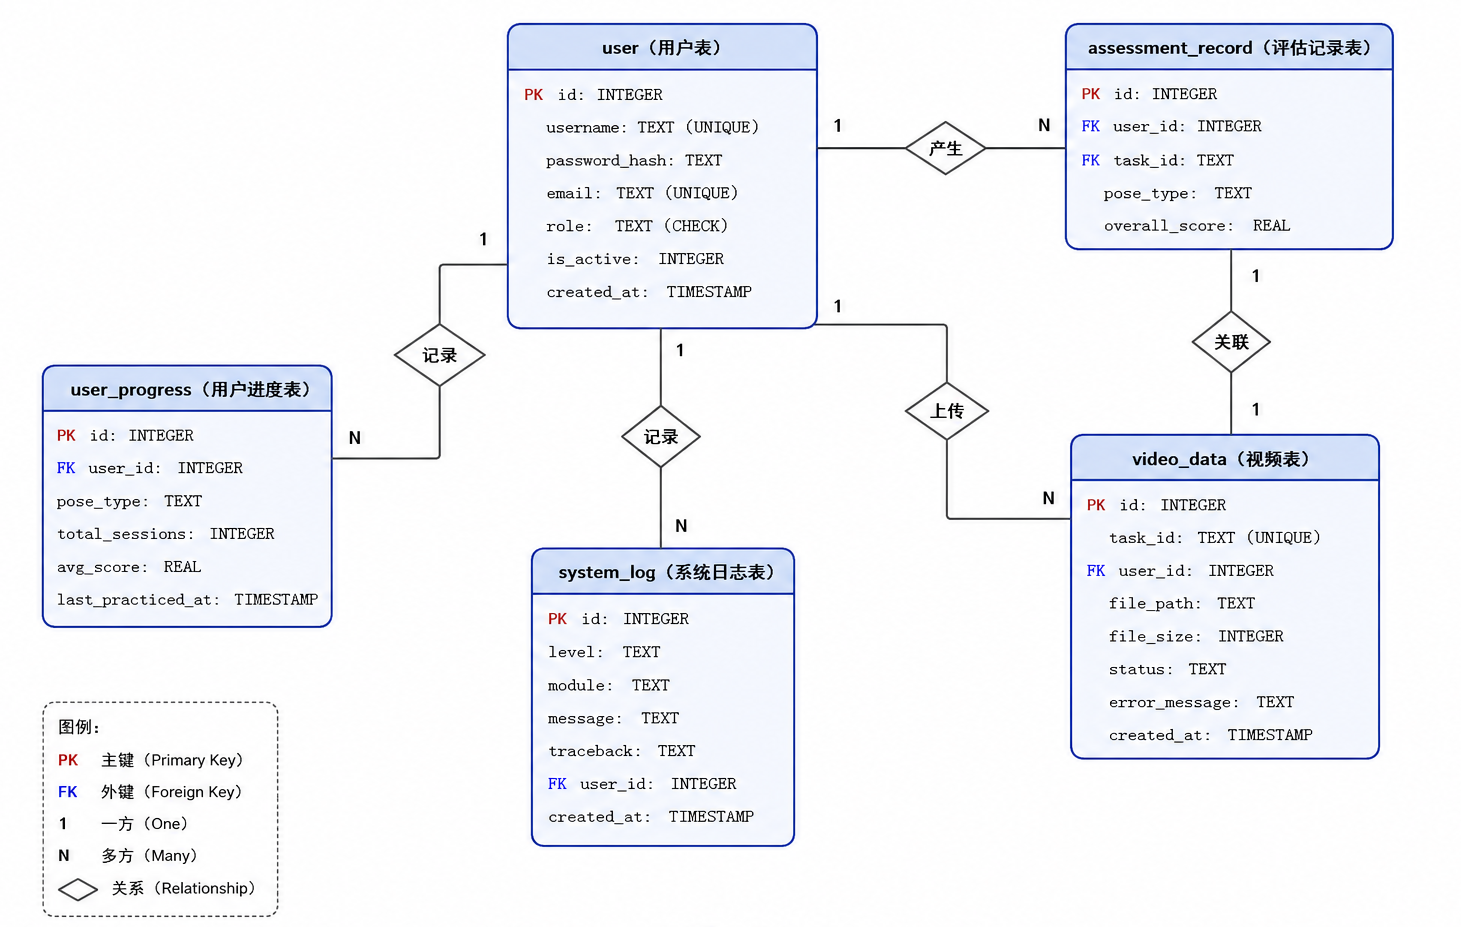
\includegraphics[width=0.96\textwidth,keepaspectratio]{../../../images/er_3.3.png}%
}

% === END INLINE: chapters/00_custom_macros.tex ===
% === BEGIN INLINE: template/template/style.tex ===
% 修复 ctex 的 \chapter 页首额外下移问题
% 原因：ctex 的 \@makechapterhead / \@makeschapterhead 开头会执行
% \vspace*{\CTEX@headingskip}，即使 beforeskip=0pt，
% 也会在页首留下额外垂直项，导致正文一级标题比声明页标题低。

\makeatletter

\def\@makechapterhead#1{%
  \begingroup
    \CTEX@heading@format@initial
    \CTEX@chapter@format{%
      \CTEX@headinghang{chapter}%
        {\CTEXifname{\CTEX@chaptername\CTEX@chapter@aftername}{}}%
      \CTEX@chapter@titleformat{#1}%
      \CTEX@chapter@aftertitle}%
  \endgroup
  \nobreak
  \CTEX@setheadingskip \CTEX@chapter@afterskip
  \ifodd \CTEX@chapter@fixskip \CTEX@fixheadingskip \fi
  \vskip \CTEX@headingskip
}

\def\@makeschapterhead#1{%
  \begingroup
    \CTEX@heading@format@initial
    \CTEX@chapter@format{%
      \CTEX@headinghang{chapter}{}%
      \CTEX@chapter@titleformat{#1}%
      \CTEX@chapter@aftertitle}%
  \endgroup
  \nobreak
  \CTEX@setheadingskip \CTEX@chapter@afterskip
  \ifodd \CTEX@chapter@fixskip \CTEX@fixheadingskip \fi
  \vskip \CTEX@headingskip
}

\makeatother

% secnumdepth=2：编号到 subsection，即模板中的三级标题
% tocdepth=2：目录显示到 subsection，即目录中显示三级标题
% 后三句：强制编号格式改成阿拉伯数字层级形式
\setcounter{secnumdepth}{2}
\setcounter{tocdepth}{2}

\renewcommand{\thechapter}{\arabic{chapter}}
\renewcommand{\thesection}{\thechapter.\arabic{section}}
\renewcommand{\thesubsection}{\thesection.\arabic{subsection}}

\ctexset{
  chapter = {
    name = {,},
    number = \arabic{chapter}
  }
}

\makeatletter
\@ifundefined{ifThesisPrintVersion}{%
  \newif\ifThesisPrintVersion
  \ThesisPrintVersionfalse
}{}
\makeatother

\newcommand{\InsertPrintBlankPage}{%
  \ifThesisPrintVersion
    \clearpage
    \thispagestyle{empty}%
    \null
    \addtocounter{page}{-1}%
    \clearpage
  \fi
}



% 使用 ctexset 对章节标题、页眉页脚等样式进行定制，以满足学校对字体和字号的要求。
% 一级标题（章标题）使用黑体、小三号字号，并居中排版；二级标题使用黑体四号；
% 三级标题使用黑体小四号；四级标题使用楷体小四号；五级标题使用宋体加粗小四号。
\ctexset{
  chapter={
    format=\centering\heiti\zihao{-3},
    nameformat=\heiti\zihao{-3},
    beforeskip=0pt,
    afterskip=17pt,
    aftername = {\;},
  },
  section={
    format=\raggedright\heiti\zihao{4},
    beforeskip=2pt,
    afterskip=3pt,
    aftername = {\;},
  },
  subsection={
    format=\raggedright\setstretch{1.5}\heiti\zihao{-4},
    beforeskip=0pt,
    afterskip=3pt,
    aftername = {\;},
  },
  subsubsection={
    format=\raggedright\setstretch{1.5}\kaishu\zihao{-4},
    beforeskip=0pt,
    afterskip=0pt,
    aftername = {\;},
  }
}

% 模板中的四级标题：编号为（1）、（2）、（3）……，楷体小四号，顶格。
\newcounter{fourthsection}[subsection]
\renewcommand{\thefourthsection}{（\arabic{fourthsection}）}
\newcommand{\fourthsection}[1]{%
  \refstepcounter{fourthsection}%
  \par\noindent{\setstretch{1.5}\kaishu\zihao{-4}\thefourthsection#1\par}%
  \nobreak
}

% 页面设置
\geometry{
  a4paper,
  top=2.9cm,
  bottom=4cm,
  left=2.5cm,
  right=2.5cm
}

% 页眉页脚位置
\setlength{\headheight}{14pt}   % 页眉区域高度，给 fancyhdr 留够空间
\setlength{\headsep}{2.01cm}    % 使页眉基线大致落在距顶边 1.5cm 附近
\setlength{\footskip}{1.0cm}    % 使页脚基线大致落在距底边 1.5cm 附近

% 页眉和页脚
\pagestyle{fancy}
\fancyhf{}

% 页眉：宋体五号（10.5pt）
\fancyhead[C]{\raisebox{4pt}{\songti\zihao{5} 成都大学本科毕业设计（论文）}}

% 页脚：宋体小五（9pt）
\fancyfoot[C]{\songti\zihao{-5}\thepage}

\renewcommand{\headrulewidth}{0.4pt}
\renewcommand{\footrulewidth}{0pt}

% 章节首页也使用相同页眉页脚
\makeatletter
\def\ps@plain{\ps@fancy}
\makeatother

% 正文字体及行距设置
\newcommand{\ThesisBodyFont}{%
  \songti\zihao{-4}%
  \linespread{1.35}\selectfont%
}

\newcommand{\ThesisBodyStyle}{%
  \ThesisBodyFont
  \setlength{\parindent}{2em}%
  \setlength{\parskip}{0pt}%
}

\makeatletter
\renewcommand{\normalsize}{\ThesisBodyFont}
\makeatother

\AtBeginDocument{%
  \ThesisBodyStyle
}

% 调研列表：编号格式为“（1）”“（2）”。
\newlist{researchlist}{enumerate}{1}
\setlist[researchlist]{%
  label=（\arabic*）,
  ref=（\arabic*）,
  labelindent=2em,
  leftmargin=*,
  labelsep=0.2778em,
  itemsep=0pt,
  topsep=0pt,
  parsep=0pt,
  partopsep=0pt
}

\newcommand{\researchitem}[2]{%
  \item #1%
  \par\begingroup
    \leftskip=-\leftmargin
    \rightskip=0pt
    \parindent=2em
    \noindent\hspace*{2em}\ignorespaces#2\unskip\par
  \endgroup
}

% 目录点线：数字越小，点越密。默认约为 4.5，这里调成接近 Word 模板的密度。
\makeatletter
\renewcommand{\@dotsep}{0.1}
\renewcommand*\l@chapter[2]{%
  \ifnum \c@tocdepth >\m@ne
    \addpenalty{-\@highpenalty}%
    {\@dottedtocline{0}{0em}{1.8em}{#1}{#2}}%
    \penalty\@highpenalty
  \fi
}

\renewcommand*\l@section{%
  \@dottedtocline{1}{2.0em}{1.8em}%
}

\renewcommand*\l@subsection{%
  \@dottedtocline{2}{4.0em}{1.8em}%
}

\makeatother


% 图题、表题格式：居中，黑体，五号。
\DeclareCaptionFont{thesiscaptionfont}{\heiti\zihao{5}}
\captionsetup{
  font=thesiscaptionfont,
  labelfont=thesiscaptionfont,
  textfont=thesiscaptionfont,
  justification=centering,
  singlelinecheck=true,
  parindent=0pt
}
\captionsetup[figure]{position=bottom, labelsep=space}
\captionsetup[table]{position=top, labelsep=space}

% 表内文字：中文宋体五号，数字和英文使用 Times New Roman。
\AtBeginEnvironment{tabular}{\songti\zihao{5}\fontspec{Times New Roman}}

% 算法块输入、输出标签。
\floatname{algorithm}{算法}
\algrenewcommand\algorithmicrequire{\textbf{输入：}}
\algrenewcommand\algorithmicensure{\textbf{输出：}}

% 浮动体内部不继承正文首行缩进，避免图片、表格和题名整体超出版心。
\AtBeginEnvironment{figure}{\setlength{\parindent}{0pt}}
\AtBeginEnvironment{table}{\setlength{\parindent}{0pt}}
\AtBeginEnvironment{algorithm}{\setlength{\parindent}{0pt}}

% 参考文献正文：宋体五号，1.25 倍行距。
\AtBeginEnvironment{thebibliography}{%
  \songti\zihao{5}%
  \linespread{1.25}\selectfont%
  \setlength{\bibsep}{0pt}%
  \setlength{\itemsep}{0pt}%
  \setlength{\parsep}{0pt}%
  \setlength{\parskip}{0pt}%
}

% 摘要页版式距离：标题、个人信息表格、正文三块之间的距离都在这里控制。
\newlength{\ChineseAbstractTitleInfoGap}
\setlength{\ChineseAbstractTitleInfoGap}{28pt}
\newlength{\ChineseAbstractInfoTextGap}
\setlength{\ChineseAbstractInfoTextGap}{1.5em}
\newlength{\EnglishAbstractTitleInfoGap}
\setlength{\EnglishAbstractTitleInfoGap}{28pt}
\newlength{\EnglishAbstractInfoTextGap}
\setlength{\EnglishAbstractInfoTextGap}{1.5em}

\newcommand{\makeAbstractTitle}[2]{%
  {%
    \centering
    #1#2\par
  }%
}

\newcommand{\makeAbstractPersonalInfo}[4]{%
  {%
    \setstretch{1.25}%
    \noindent\hspace*{\abstractPersonalInfoIndent}% 摘要处个人信息左边距
    \begin{tabular}{@{}>{\kaishu\zihao{-4}}l@{\hspace{\abstractPersonalInfoColumnGap}}>{\kaishu\zihao{-4}}l@{}}
      专业：#1 & 学\hspace{2em}号：\TNR{#2} \\[1.25em]
      学生：#3 & 指导教师：#4
    \end{tabular}\par
  }%
}

\newcommand{\makeChineseAbstractHeader}[5]{%
  \clearpage
  \makeAbstractTitle{\setstretch{1.5}\heiti\zihao{-2}}{#1}%
  \vspace{\ChineseAbstractTitleInfoGap}
  %\addcontentsline{toc}{chapter}{摘要}
  \makeAbstractPersonalInfo{#2}{#3}{#4}{#5}
  \vspace{\ChineseAbstractInfoTextGap}
}

\newcommand{\ChineseAbstractTextStart}{%
  \noindent {\heiti\zihao{-4} 摘要}：\begingroup\songti\zihao{-4}\ignorespaces
}

\newcommand{\ChineseAbstractTextFinish}{%
  \endgroup
}

\newcommand{\makeChineseKeywords}[1]{%
  \par\vspace{\baselineskip}\noindent{\heiti\zihao{-4} 关键词：}\,{\songti\zihao{-4} #1}
}

\newcommand{\makeEnglishAbstractPersonalInfo}[4]{%
  {%
    \setstretch{1.25}%
    \noindent\hspace*{\englishAbstractPersonalInfoIndent}%
    \begin{tabular}{@{}>{\fontspec{Times New Roman}\zihao{-4}}l@{\hspace{\englishAbstractPersonalInfoColumnGap}}>{\fontspec{Times New Roman}\zihao{-4}}l@{}}
      Major：#1 & Student ID：\TNR{#2} \\[1.5em]
      Student：#3 & Instructor：#4
    \end{tabular}\par
  }%
}

\newcommand{\makeEnglishAbstractHeader}[5]{%
  \clearpage
  \makeAbstractTitle{\setstretch{1.25}\fontspec{Times New Roman}\bfseries\zihao{-2}}{#1}%
  \vspace{\EnglishAbstractTitleInfoGap}
  \makeEnglishAbstractPersonalInfo{#2}{#3}{#4}{#5}
  \vspace{\EnglishAbstractInfoTextGap}
}

\newcommand{\EnglishAbstractTextStart}{%
  \noindent {\fontspec{Times New Roman}\bfseries\zihao{-4} Abstract}:%
  \begingroup\fontspec{Times New Roman}\zihao{-4}\setlength{\parindent}{2em}\ignorespaces
}

\newcommand{\EnglishAbstractTextFinish}{%
  \endgroup
}

\newcommand{\makeEnglishKeywords}[1]{%
  \par\vspace{\baselineskip}\noindent{\fontspec{Times New Roman}\bfseries\zihao{-4} Key words:}\,{\fontspec{Times New Roman}\zihao{-4} #1}
}
% === END INLINE: template/template/style.tex ===
% === BEGIN INLINE: chapters/00_local_defs.tex ===
\newcommand{\abstractPersonalInfoIndent}{5em}
\newcommand{\abstractPersonalInfoColumnGap}{12em}
\newcommand{\englishAbstractPersonalInfoIndent}{5em}
\newcommand{\englishAbstractPersonalInfoColumnGap}{3em}

\newcommand{\thesisTitleLineA}{基于多模态大模型的}
\newcommand{\thesisTitleLineB}{瑜伽动作评估系统}
\newcommand{\thesisCollege}{计算机学院}
\newcommand{\thesisMajor}{计算机科学与技术}
\newcommand{\thesisMajorEn}{Computer Science and Technology}
\newcommand{\studentName}{曹黎骏}
\newcommand{\studentNameEn}{Cao Lijun}
\newcommand{\studentId}{202210305212}
\newcommand{\studentClass}{计科1班}
\newcommand{\advisorName}{张楗伟}
\newcommand{\advisorNameEn}{Jianwei Zhang}
\newcommand{\advisorTitle}{讲师}
\newcommand{\thesisCompletionDate}{2026 年 \quad 3 月 \quad 23 日}
\newcommand{\authorSignature}{曹黎骏}
\newcommand{\advisorSignature}{张楗伟}
\newcommand{\thesisDeclarationDate}{2026 年 3 月 23 日}

\newcommand{\listbodyaligntext}[1]{%
  \par\begingroup
    \leftskip=-\leftmargin
    \rightskip=0pt
    \parindent=2em
    \noindent\hspace*{2em}\ignorespaces#1\unskip\par
  \endgroup
}

% === END INLINE: chapters/00_local_defs.tex ===

\begin{document}

% === BEGIN INLINE: template/template/cover.tex ===
\newlength{\labelwd}      % 左侧标签列宽
\newlength{\fullwd}       % 整行下划线宽度
\newlength{\leftlinewd}   % 学号/指导教师 下划线宽度
\newlength{\rightlinewd}  % 班级/职称 下划线宽度
\newlength{\midlabelwd}   % 班级/职称 标签列宽

\setlength{\labelwd}{2.43cm} % Word 模板左侧标签列宽
\setlength{\fullwd}{10.5cm}  % Word 模板整行下划线列宽
\setlength{\leftlinewd}{4.76cm}
\setlength{\midlabelwd}{1.50cm}
\setlength{\rightlinewd}{3.77cm}

\newcommand{\coverLabelFont}{\heiti\fontsize{18pt}{22pt}\selectfont}
\newcommand{\coverValueFont}{\heiti\fontsize{16pt}{20pt}\selectfont}


\newcommand{\coverline}[2]{%                             % 封面下划线格式
  \makebox[#1][c]{%
    \ooalign{%
      \hfil{\coverValueFont #2}\hfil\cr
      \smash{\raisebox{-4.5pt}{\rule{#1}{0.4pt}}}\cr     % 文字位置不变，将下划线往下移动4.5pt
    }%
  }%
}
\newcommand{\covertwolabel}[2]{%
  {\coverLabelFont\makebox[\labelwd][l]{#1\hspace{2.0em}#2}}%
}
\newcommand{\coverlabel}[1]{%
  {\coverLabelFont\makebox[\labelwd][l]{#1}}%
}
\newcommand{\covermidlabel}[1]{%
  {\coverValueFont\makebox[\midlabelwd][c]{#1}}%
}

\newcommand{\coverTitleFont}{\CJKfontspec[Path=../../templates/CDU_thesis_latex/fonts/]{msyhbd-title.ttf}}

\begin{titlepage}
  \thispagestyle{empty}
   \begin{center}
	   \vspace*{-26pt}
	   
\includegraphics[width=10.72cm,height=3.25cm]{figs/cdu.pdf}

		    \vspace{25pt}
    % 封面主标题使用微软雅黑加粗，按 Word 模板视觉放大。
    {\coverTitleFont\fontsize{42pt}{50pt}\selectfont 本科毕业设计（论文）}\\[3.3cm]
    % 题目等信息：标签 18pt，填写内容 16pt。
    {
    \begin{tabular}{@{}c@{\hspace{0.55cm}}c@{}c@{}c@{}}
      \covertwolabel{题}{目} & \multicolumn{3}{c@{}}{\coverline{\fullwd}{\thesisTitleLineA}}\\[1.7em]
      & \multicolumn{3}{c@{}}{\coverline{\fullwd}{\thesisTitleLineB}}\\[1.7em]

      \covertwolabel{学}{院} & \multicolumn{3}{c@{}}{\coverline{\fullwd}{\thesisCollege}}\\[1.7em]

      \covertwolabel{专}{业} & \multicolumn{3}{c@{}}{\coverline{\fullwd}{\thesisMajor}}\\[1.7em]

      \coverlabel{学生姓名} & \multicolumn{3}{c@{}}{\coverline{\fullwd}{\studentName}}\\[1.7em]

       \covertwolabel{学}{号} & \coverline{\leftlinewd}{\studentId} & \covermidlabel{班级} & \coverline{\rightlinewd}{\studentClass}\\[1.7em]

      \coverlabel{指导教师} & \coverline{\leftlinewd}{\advisorName} & \covermidlabel{职称} & \coverline{\rightlinewd}{\advisorTitle}\\[1.7em]

      \coverlabel{完成时间} & \multicolumn{3}{c@{}}{\coverline{\fullwd}{\thesisCompletionDate}}\\
    \end{tabular}
    }
  \end{center}

\end{titlepage}
% === END INLINE: template/template/cover.tex ===
% === BEGIN INLINE: template/template/declarations.tex ===
\newcommand{\heitchapter}[1]{%
  \clearpage
  \begin{center}
    {\setstretch{1.5}\heiti\zihao{-2}#1\par}
  \end{center}
  \vspace{12pt}%
}

% 成大论文模板要求1.25倍行距，宋体，小三号，这里经过像素级对比使用1.3倍行距保证视觉效果一致
\newcommand{\declarationbodyfont}{%
  \setstretch{1.30}\songti\zihao{-3}%
}

\newcommand{\signaturefield}[1]{%
  \makebox[8em][l]{#1}%
}

% 声明页不参与前置部分的罗马页码编号；罗马页码从摘要开始。
\pagenumbering{gobble}

% 原创性声明
%\chapter*{{\heiti\zihao{-2} 原创性声明}}
\heitchapter{原创性声明}
%\addcontentsline{toc}{chapter}{原创性声明}
% 原创性声明正文使用宋体小三号，1.25倍行距
{\declarationbodyfont

\indent 本人郑重声明：本人所呈交的毕业设计（论文），是在指导老师的指导下独立进行研究所取得的成果。毕业设计（论文）中凡引用他人已经发表或未发表的成果、数据、观点等，均已明确注明出处。除文中已经注明引用的内容外，不包含任何其他个人或集体已经发表或撰写过的科研成果。对本文的研究成果做出重要贡献的个人和集体，均已在文中以明确方式标明。\\

\indent 本声明的法律责任由本人承担。\\[2ex]

\indent 论文作者签名：\signaturefield{\authorSignature} 日\quad 期：\thesisDeclarationDate\\
%\indent 论文作者签名：\signaturefield{} 日期：\\
}% 结束宋体小三号设置

\InsertPrintBlankPage

% 使用授权声明
%\chapter*{{\heiti\zihao{-2} 关于使用授权的声明}}
\heitchapter{关于使用授权的声明}
%\addcontentsline{toc}{chapter}{关于使用授权的声明}
% 使用授权声明正文使用宋体小三号，1.25倍行距
{\declarationbodyfont

\indent 本人在指导老师指导下所完成的毕业设计（论文）及相关的资\nobreak 料\nobreak（包括图纸、试验记录、原始数据、实物照片、图片、录音带、设计手稿

\noindent 等），知识产权归属成都大学。本人完全了解成都大学有关保存、使用毕业设计（论文）的规定，本人授权成都大学可以将本毕业设计\nobreak（论文）的全部或部分内容编入有关数据库进行检索，可以采用任何复制手段保存和汇编本毕业设计（论文）。如果发表相关成果，一定征得指导教师同意，且第一署名单位为成都大学。本人离校后使用毕业设计\nobreak（论文）或与该论文直接相关的学术论文或成果时，第一署名单位仍然为成都大学。

\indent 本毕业设计（论文）内容不涉及国家秘密、商业秘密及其他需要保密的内容，适用于上述授权。\\

%\indent 论文作者签名：\signaturefield{} 日期：\\
\indent 论文作者签名：\signaturefield{\authorSignature} 日\quad 期：\thesisDeclarationDate\\

\indent 指导教师签名：\signaturefield{\advisorSignature} 日\quad 期：\thesisDeclarationDate \\
}% 结束宋体小三号设置

\InsertPrintBlankPage

\clearpage
% === END INLINE: template/template/declarations.tex ===
% === BEGIN INLINE: chapters/01_abstracts.tex ===
\makeChineseAbstractHeader
  {基于多模态大模型的瑜伽动作评估系统}
  {计算机科学与技术}
  {202210305212}
  {曹黎骏}
  {张楗伟}
\ChineseAbstractTextStart
本文面向居家瑜伽练习中的动作评估问题展开研究。居家练习者虽然可以跟随视频完成体式，但往往难以判断关节角度、身体对齐和动作稳定性是否达到要求。线下教练能够提供即时纠正，却受到时间、地点和费用限制，因此有必要构建一套可反复使用、反馈清晰且便于留存的辅助评估工具。

围绕这一需求，本文设计并实现了一套基于多模态大模型的瑜伽动作评估系统。系统采用前后端分离架构，前端基于HTML、CSS和原生JavaScript实现注册登录、视频上传、任务轮询与结果展示；后端以Flask提供RESTful接口，并使用SQLite存储用户信息、视频任务、评估记录与系统日志。算法层以MediaPipe Pose提取视频中的33个人体关键点，再通过OpenCV和时序统计计算关节角度、身体对齐偏差与动作稳定性等结构化特征。

在评估方法上，系统保留本地规则评估模块，用于完成基础打分和问题定位，再将关键帧、规则结果与结构化特征发送给千问多模态模型，生成更自然的反馈文本和改进建议。该设计兼顾结果可解释性与模型表达能力，并能在网络服务不稳定时提供降级输出。

最终系统完成了注册、登录、视频上传、后台异步处理、状态查询、结果回显和历史记录留存等主要链路。测试表明，系统能够在本地环境下完成从视频输入到评估反馈的完整流程，并在部分异常场景下保持基本可用，形成了一套可运行、可验证且可继续扩展的毕业设计原型。
\ChineseAbstractTextFinish
\makeChineseKeywords{瑜伽动作评估；多模态大模型；Flask框架；前后端分离；姿态估计}

\makeEnglishAbstractHeader
  {Yoga Action Assessment System Based on Multimodal Large Language Models}
  {Computer Science and Technology}
  {202210305212}
  {Cao Li Jun}
  {Zhang Jian Wei}
\EnglishAbstractTextStart
This thesis addresses a practical problem in home yoga training: learners may follow a pose video, but they still cannot easily judge whether their movement is aligned well enough. To deal with this issue, the project implements a yoga action assessment system that combines pose estimation, rule-based analysis, and multimodal language feedback.

The system uses a frontend-backend architecture. The frontend is built with HTML, CSS, and vanilla JavaScript for upload, polling, and result display. The backend is implemented with Flask framework, and SQLite database is used to store user data, task records, assessment results, and logs. In the analysis stage, MediaPipe Pose algorithm extracts 33 body landmarks from video frames, and OpenCV geometric calculations are then used to derive joint angles, alignment deviation, and motion stability features.

For evaluation, the project keeps a local rule-based scoring mechanism as the baseline and uses the Qwen multimodal model to convert structured errors and keyframe information into readable corrective suggestions. This design also makes fallback possible when the external model service is unstable. During development, several engineering issues were handled, including API field mismatch, SQLite locking, blocking processing, and proxy interference. The final system can complete the main assessment workflow on a local machine and generate usable feedback for yoga practice.
\EnglishAbstractTextFinish
\makeEnglishKeywords{Yoga Action Assessment; Multimodal Large Language Model; MediaPipe; Flask; Frontend-Backend Separation; Pose Estimation}
% === END INLINE: chapters/01_abstracts.tex ===

% 目录
\clearpage
\begin{center}
  {\songti\zihao{-2}\bfseries 目录}
\end{center}
\vspace{1.5em}

\makeatletter
\@starttoc{toc}
\makeatother

% 正文开始，使用阿拉伯数字编号
\clearpage
\pagenumbering{arabic}

% === BEGIN INLINE: chapters/02_mainmatter.tex ===
% 第一章 绪论
\chapter{绪论}

\section{课题背景}
近几年，居家健身因其便利性和经济性而越来越普遍。瑜伽也从一项兴趣爱好，变成很多人长期要坚持的一项日常训练。它和以前那种以心肺负荷为主的锻炼方式不同，瑜伽更讲究动作的完成度，也更讲究身心的控制程度。练习者不仅要把体式摆出来，还要注意肩、髋、膝、踝、脊柱是否在合理的点位上，呼吸和发力顺序是否在配合着。如果基础条件都没有把握好，动作可能看起来和标准型没有多大出入，但是训练收益往往是有限的，时间一长反复也会诱发代偿和损伤。

在真实场景里，很多人的困难不是“跟不上动作”，而是“无法判断自己做得准不准”。初学者对身体角度、关节排列缺乏稳定感知。居家练习，很多时候都是看着教学视频做形状。镜子视角小，手机回放又很难拉慢放指指出问题所在。一个动作是膝盖超伸了，还是骨盆前倾了，或者肩膀发力次序出问题了，练习者自己很难分辨。而问题始终得不到纠正的话，在重复练习中就会固化错误姿势。

线下教练能给予及时的反馈，这是传统教学方式最直接的优势。但这样的方式也有一个现实的边界，课程时间要合二为一，场地并不总是便利，长期上课也要负担一笔不小的费用。更关键的是，很多纠正意见停留在课堂当下，当练习者回到家里以后，依旧缺少一套可以随时复看反复比较留下记录的量化依据。也正因为如此，居家场景并不只是一个缺“能看动作”的工具，而是缺一套“能说明哪里有问题、为什么有问题、怎样调整”的辅助系统。

而计算机视觉、姿态估计、多模态模型的发展，让这个问题有了可以落地实施的技术路线，相关中文综述也表明，深度学习姿态估计和视觉语言预训练正在从单一识别逐步走向结构化理解与交互反馈\cite{ref_cn_pose_estimation_survey,ref_cn_visual_language_pretraining}。工程实现上，系统使用Flask框架\cite{ref_flask}构建后端接口，并采用SQLite数据库\cite{ref_sqlite}保存用户、视频任务、评估记录与系统日志；算法链路上，MediaPipe姿态估计算法\cite{ref_mediapipe}能够比较稳定地抽取出视频中的33个关键点，加上OpenCV\cite{ref_opencv}几何计算，系统就可以获得输出的关节和角度、对齐、动作稳定性等指标；在反馈生成阶段，系统再将结构化特征和关键帧信息交给千问多模态模型\cite{ref_qwen}处理，使其具备把“数字结果”翻译成更贴近日常教学语言的反馈文本的机会。基于这个背景，本文将以“基于多模态大模型的瑜伽动作评估系统”作为毕设题目，完成了一套可以运行、能够联调、能够保存结果和支撑论文论证的工程原型。

\section{国内外研究现状}
动作识别、姿态评估是计算机视觉领域的重要研究方向。在该领域，围绕这个方向，其实已经研究了很久。国内关于视频人体动作识别的研究综述指出，动作识别方法已经从传统手工特征逐渐发展到深度网络、时序建模和骨架序列建模等路线\cite{ref_cn_video_action_survey}。Andriluka等人\cite{ref_mpii}建立的MPII人体姿态数据集至今仍是该领域重要的基准测试资源。Wei等人\cite{ref_cpm}提出的卷积姿态机通过多阶段细化有效提升了姿态估计精度。Chen等人\cite{ref_cpn}提出的级联金字塔网络则在处理遮挡和多人场景方面表现优异。Saraf等人\cite{ref_har_survey}对基于深度学习的人体活动识别方法进行了系统综述，总结了从骨架序列到时空图卷积等多种技术路线。Singh等人\cite{ref_lstm_pose_action}则探索了利用LSTM网络从姿态序列中进行动作识别的方法。这些研究为瑜伽动作识别与评估提供了重要的技术基础和方法参考。以前更多关注的是“人在做什么动作”。而后来更多关注的是“这个动作做得是否规范”。这两个问题看着很接近，但难易程度其实是有区别的。前者偏分类。而后者不仅要识别动作，还要解释偏差、定位问题和给出反馈，所以对算法、规则、输出形式的要求都更高。

如果只看底层姿态感知，现阶段已经有开发较为成熟的开源工具可以利用，早先的手段更多地依赖人为主观设计特征的图像方法和几何模型。他们对于背景复杂或人体遮挡情况或是光照不稳定等方面的鲁棒性往往较差，OpenPose\cite{ref_openpose}之后的多人姿态的检测能力有了较为明显的提升，但它对算力的需求也更高，普通的开发机部署与调试的成本也相对更多。Newell等人\cite{ref_hourglass}提出的堆叠沙漏网络和Xiao等人\cite{ref_simple_baselines}提出的Simple Baselines方法在人体姿态估计领域取得了显著进展，其中Simple Baselines以其简洁的网络结构在精度和速度之间取得了较好平衡。而Zheng等人\cite{ref_pose_survey}的综述研究则系统梳理了深度学习时代人体姿态估计技术的发展脉络。本文调研发现，瑜伽动作识别方向也有学者开展过相关工作，如Zhang等人\cite{ref_yoga_recognition}和Field等人\cite{ref_yoga_pose_estimation}分别从视频分析和姿态估计角度对瑜伽动作进行了识别与校正研究。而MediaPipe姿态估计算法\cite{ref_mediapipe}似乎更适合本文这种以本地验证与落地工程为主的课题，它基于BlazePose架构，输出33个关键点，模型的推理速度也适合在普通PC环境下部署，被广泛地应用在需要轻量化的人体姿态分析的场景。

再看评估层面，根据公开资料、开发记录和现有开源实践，相关方法大致可以分为下面三类:
\begin{researchlist}
  
\researchitem{规则驱动评估}{
    系统提取关键点后，再计算肘、膝、髋、肩等关节的角度，把结果与系统设定好的标准进行比较。它的优点很明显是实现了直接驱动。打分依据很直接，也便于解释扣分的原因。而它的缺点也能很明显地看出来。不同的练习者的体型、柔韧性、拍摄的角度等并不是统一的，一成不变的阈值很容易造成误判，反馈的文本通常比较生硬。
  }
  
\researchitem{端到端学习评估}{
    这类方法一般收集带有评分标签的视频或骨架序列，再学习时空模型直接输出动作分值，它在复杂场景下有较好的整体拟合能力，但往往可解释性较差。用户看到分数后依然容易不知道是哪一个关节、哪一段动作或者哪一种发力方式出现问题。
  }
  
\researchitem{多模态联合评估}{
    这个角度是近两年更多人关注的一个角度，尝试将视频关键帧，姿态序列和结构化特征同时交给多模态模型，然后输出自然语言的评价语。国内视觉语言多模态预训练综述对图文对齐、跨模态融合和下游任务迁移进行了系统梳理，也说明多模态模型具备把视觉信息与文本语义共同建模的技术基础\cite{ref_cn_visual_language_pretraining}。Papadopoulos等人\cite{ref_multimodal_concept}在跨领域多模态概念检测方面的研究为多模态特征融合提供了重要参考，Horn\cite{ref_pose_hierarchy}关于层次化姿态估计的综述研究则从另一个视角梳理了姿态感知技术的发展脉络。Rich等人\cite{ref_3d_pose_tracking}在3D人体姿态估计与跟踪方面的工作进一步拓展了姿态分析的维度。其特点是表达能力更强，更贴合日常的教学场景，但会涌现更多新的问题，例如：提示语词设计，输出格式控制，接口稳定性问题，成本问题。
  }
\end{researchlist}

对本课题来说，更实际的目标不是做一个“能够识别出动作名称”的展示程序，而是把识别结果继续落到评分、解释和建议上。瑜伽场景对细节有着相当的要求，做了一个系统，对于用户来说，只能判断出他做的究竟是什么体式，对其中偏差出现在什么部位、应当怎样调整什么动作都无法解释的话，对真实的练习并没有什么帮助。在判断下，本文最终选择把姿态提取、几何规则分析和多模态反馈放到同一套系统里做，用工程的方式完成一次相对完整的尝试。

\section{面临的问题与挑战}
把一个“视频分析加模型反馈”的想法做成可交互、可演示、可保存结果的Web系统的难点其实不只在算法，很多问题在原型阶段看不到，等前端、后端、数据库、外部模型服务等全部搭起来后，就会出现新的工程压力。结合领域经验，主要有以下几方面的挑战：
\begin{researchlist}
  
\researchitem{动作标准难以固定}{
    同一个体式，不同练习者的身高、体量和柔韧性都会有差异。规则若是僵硬的，系统会轻易地把合理动作判断为错误动作。规则若是较弱的，评估又会失去压力。
  }
  
\researchitem{居家视频质量不稳定}{
    居家拍摄视频往往存在光线阴暗、背景杂物多、机位随意和局部遮挡的情况，同时瑜伽肢体动作本身存在很多肢体交叠的情况，以上条件下关键点检测模型更容易漂移，且置信度更差。
  }
  
\researchitem{规则结果不等同于用户能看懂的反馈}{
    几何计算能给出角度的偏差，但用户需要的不只是“差了多少度”，他想知道问题出在哪个部位、为什么会这样、练习时应该怎么调整，单靠规则判断很难把这个表达得足够自然。
  }
  
\researchitem{外部模型服务不可控}{
    大模型接口可能存在代理变量、网络波动、请求超时、返回格式异常的扰动因素，实际项目中就遇到过联调时真实环境代理环境变量导致请求异常阻断的问题，如果系统没有容错和降级机制，就会把主流程拖住，变成单点故障。
  }
  
\researchitem{多模块联动容易暴露工程故障}{
    视频解码、姿态识别、数据库写入、线程调度、前端轮询存在较为明显的耦合。开发记录中存在过上传同步阻塞、接口字段不一致、\texttt{no such column: user\_id} 触发器错误，以及 \texttt{NoneType is not iterable} 等问题，可见整条链路真正稳定下来并不是一件容易的事。
  }
\end{researchlist}

把这些问题放在一起看，你会发现该课题真正难的不是某一个单点模块，而是串接起来之后是否还能继续工作。也正是因为这样，该文在实现阶段关注的不是某一个局部指标，而是整条业务能否跑通，结果能否解释，异常能否兜底。

\section{主要工作内容}
本文在现有的姿态估计算法的基础上进行创新，将其融合成一个综合评估系统，重点在于系统集成、流程打通和工程实现。本文探讨了如何才能把已有的姿态提取方法、规则分析思路和多模态反馈能力组织成一套能运转的工程实践。围绕这个目的，本文完成的主要工作有：
\begin{researchlist}
  \researchitem{用户需求梳理}{
    根据居家练习场景进行用户需求梳理，梳理普通用户和管理员这两类角色权限边界、输入方式和结果呈现目标
  }
  \researchitem{关键点提取}{
    采用MediaPipe姿态估计算法\cite{ref_mediapipe}完成对视频帧的人体关键点的提取，形成后续角提取和稳定性判定算法的数据支撑
  }
  \researchitem{特征计算模块}{
    设计基于几何关系和时序统计计算的特征计算模块，对关键关节角度、左右对齐关系、动作波动情况进行计算量化
  }
  \researchitem{规则评估模块}{
    构建本地规则评估模块，依托动作标准库实现基础打分、问题定位、降级输出
  }
  \researchitem{千问模型接入}{
    接入千问模型，针对提示词、结构化返回、错误解析机制进行多轮调试，让反馈文本更贴近日常教学语言
  }
  \researchitem{业务链路实现}{
    完成注册登录、上传视频、后台异步任务、轮询查询、结果回显、历史记录等主要业务链路
  }
  \researchitem{故障修复}{
    定位并修复对联调中出现的真实故障，如前后端字段不匹配、角色字段映射冲突、数据库锁冲突、触发器列引用错误、空对象迭代异常、代理变量造成的模型请求失败
  }
\end{researchlist}



\section{论文组织结构}论文整体按照“问题提出、需求拆解、系统设计、实验验证”来展开，其中：第一章为绪论，阐述课题的背景、相关研究现状、项目存在的主要问题和论文针对该问题的工作内容，第二章为系统需求阐述，从角色划分、功能模块、性能需求三个角度阐述系统需要解决什么问题，第三章主要对系统架构演进、运行环境、重要实现链路和实现的数据库设计、业务时序做了阐述，是本论文的实现重点，第四章对于提出并通过具体真实的联调对系统做了功能、异常与对故障的测试分析，正文之后依次为本文的结论部分、参考文献与致谢。


% 第二章 系统需求分析
\chapter{系统需求}

\section{系统角色}
权限边界是否清晰，会直接影响到Web系统是否可以稳定地运行，所以需求分析第一步要把角色定义清晰。结合本项目的使用方式，系统内的角色主要有两类，一类是普通用户，一类是管理员，两者共享一套后端服务，但是能访问的页面、能进行的操作、能看见的数据范围都不一样。

\textbf{普通用户}：普通用户是系统的主要使用者，是整套业务流程的主要完成者。典型操作包括注册登录、瑜伽体式选择、训练视频上传、分析任务提交、处理进度查看、评估结束后的评分建议查看。还需要经常查看历史用来在前后不同时期做比较。对这类用户来说，功能多少不是需求重点，能否一目了然，等待过程是否可感知，失败原因能否说明白。换句话说，就是后台的处理过程前端必须做隐藏处理，呈现出来的东西必须是有帮助的练习信息。

\textbf{管理员}：管理员的职责更偏向于平台维护和运行监控。相较于普通用户，管理员既要能查看数据的统计，了解注册人数、评估次数、动作热度、平均分等平台层面的信息；同时也要能在必要时管理用户状态，如调整角色、禁用异常账号等。管理员不是多一个界面而已，而是意味着系统要对高权限操作进行更严格的认证和拦截。

这样的角色划分有两个好处，一是可以让普通用户界面保持尽量简洁，二是让后台管理与日常使用分离，减少权限混乱带来的安全风险。

从真实使用过程看，普通用户和管理员虽然共用同一套服务端程序，但二者关注的信息粒度完全不同。普通用户更关心单次练习是否顺利完成、分数是否容易理解、建议是否能指导下一次动作调整；管理员更关心系统是否稳定、任务是否堆积、异常是否能够追踪、用户数据是否存在越权访问风险。因此系统不能只在页面入口上区分角色，还需要在接口层和数据库查询层同时完成限制。比如普通用户访问历史记录时，只能读取自己名下的评估记录；管理员访问统计页面时，则需要读取汇总数据，但仍不应直接暴露用户密码哈希、模型原始响应等敏感内容。

角色设计还影响到错误处理方式。普通用户遇到失败时，需要看到的是“视频格式不支持”“分析超时，请稍后重试”这类可理解提示；管理员则需要在日志中看到更具体的异常类型、任务编号和发生阶段。若系统只返回底层异常文本，普通用户会难以理解；若系统只返回模糊提示，管理员又无法排查问题。因此本文在需求分析阶段就把角色和信息可见性联系起来考虑，保证同一个故障在不同角色侧有不同粒度的呈现。

此外，角色权限也是后续系统扩展的基础。若未来加入教师端或教练端，系统可以在现有普通用户和管理员之间增加新的中间角色，例如允许教练查看所负责学员的训练记录，但不允许修改全局配置和用户权限。当前项目虽然只实现了两类角色，但通过明确的鉴权中间件和接口边界，已经为后续角色扩展预留了方向。

\section{系统功能}

系统功能并不是把几个页面机械地拼在一起，而是围绕“用户怎样完成一次完整评估”来组织业务流程。结合本文的实现目标，系统功能主要拆为用户管理、视频上传、姿态多维特征提取、混合智能评估、结果展示和历史记录留存六个部分，前后联系强，基本覆盖从输入到输出的完整链路。

从用户操作路径来看，一次完整评估通常经历五个阶段：用户先完成登录，随后选择或录制瑜伽动作视频，上传后等待系统分析，分析完成后查看评分与建议，最后在历史记录中保留本次结果用于后续对比。这个流程看似简单，但其中每一步都对应后台不同模块的协作。登录阶段依赖身份认证和权限判断；上传阶段依赖文件校验和任务创建；分析阶段依赖视频处理、姿态估计和规则计算；反馈阶段依赖模型调用和结果解析；历史阶段则依赖数据库持久化和查询接口。正因为流程跨越多个模块，系统功能设计不能只罗列页面按钮，而要围绕完整闭环组织。

功能模块之间也存在明显的依赖关系。没有用户管理，就无法把评估记录归属到具体用户；没有异步任务，就无法让视频分析在较长时间内保持前端可响应；没有规则评估，就无法在模型不可用时提供兜底结果；没有历史记录，系统就只是一种一次性演示工具，而不是可持续使用的训练辅助工具。因此本文在功能分析中把这些模块作为一条连续链路，而不是孤立功能点。这样的划分更符合项目实际，也能解释为什么某些看似“后台”的模块对用户体验同样重要。

在功能实现优先级上，本文优先保证主链路可跑通，再逐步补充管理端、日志、异常兜底和可视化细节。原因在于，毕业设计阶段最重要的是证明核心方案成立：用户上传视频后，系统能够完成分析并返回有意义的反馈。如果一开始把大量精力投入装饰性页面或复杂统计面板，主链路不稳定时反而难以支撑论文论证。因此系统开发采用了“先闭环、后完善”的策略，先完成最小可用流程，再围绕联调中暴露的问题持续补强。

\subsection{用户管理}
账户体系是系统运行的基础，所以用户管理模块首先要解决完整性和安全性问题。用户注册时，提交用户名或邮箱以及密码。后端要完成唯一性校验，还不能让密码以明文进入数据库，所以系统采用 Bcrypt 对密码做加盐哈希再保存，这样即便数据库数据泄露，原始密码也不容易被复原。

在鉴权机制上，由于系统采用前后端分离架构，鉴权机制不再使用传统的Session/Cookie，而是采用JSON Web Token（JWT）\cite{ref_jwt}作为统一身份凭证。用户登录成功后，后端生成token，token包含身份、角色、过期时间等信息。前端在后续请求中通过Authorization头携带token，后端再进行校验与权限判断，这种方式更加符合RESTful接口风格，也便于前端独立部署。

开发过程中用户管理模块还暴露出典型的接口契约问题，即前后端对于角色字段命名并不统一，例如前端为了显示更直观，对于学员角色使用learner表示，而数据库层的CHECK约束只有user和admin两种值，这样在联调时就会直接导致注册失败。修复后系统在接口层增加了字段映射，使得显示层语义和数据库约束保持一致。

\subsection{视频上传}
视频上传模块是整套系统真正的业务入口，也是最容易暴露性能问题的环节。系统目前支持的格式为MP4、MOV、AVI、WebM，这些是视频网站比较常见的格式。在前端选择好视频并标注好动作后即可发起上传。由于后续还要执行抽帧、姿态推理、规则分析和模型调用，整个处理链路通常需要明显长于普通接口请求的时间，所以在这里不能采取同步阻塞的方式，否则前端会长时间无响应。

上传接口只做三件事，接收文件保存到安全目录、在数据库插入一条状态为processing的任务、返回唯一的任务编号给前端。真正的工作由后台的异步线程来分析，耗时比较长。前端再轮询单独跟踪任务的状态。接口可以尽快返回，前端页面不会长时间卡住，用户也能持续看到任务进展。

\subsection{姿态多维特征提取}
姿态特征提取是算法部分。系统最后是否有依据说断话，很大程度上取决于提供给系统的输入数据是否是稳定的、是否是有意义的。视频本身是一个片段连续像素的集合，并不是给人们提供直接打分的信息，算法系统需要先把原始画面转化成结构化的人体姿态数据。已有面向健身行为的人体姿态估计与动作识别研究也表明，骨架关键点、关节角度和动作时序特征可以较好支撑运动行为识别与规范性分析\cite{ref_cn_fitness_pose_action}。

具体来讲，这步做完至少有三层内容，第一层，抽帧、废帧过滤，尽量去掉准备动作、空画面、镜头变动阶段，第二层，解算颈、肩、肘、腕、髋、膝、踝等骨干节点三维坐标与置信度，作为下一步计算的根据地，第三步，在原始坐标基础上继续构造二级特征，比如大腿小腿夹角、左右骨盆的水平偏差，躯干倾斜程度等等，比起坐标，好对应到真实体式问题。

瑜伽评估并非判断某一帧是否“摆到了位”就可以，接下来要考虑动作维持阶段是否稳定，所以系统还对动作持续过程做了一些时序统计，比如角度波动、稳定性指标的计算，用来判断维持动作阶段的控制能力。

\subsection{混合智能评估}
评估报告最终是给用户直接阅读的，因此，系统没有只保留一个总分，而是沿用混合评估的思路，将本地规则系统和多模态模型结合起来使用。大语言模型研究综述指出，这类模型在自然语言理解、生成和指令跟随方面表现出较强能力，但也需要通过提示约束、结构化输出和异常处理降低不可控性\cite{ref_cn_llm_survey}。

其中规则系统要给出量化结果是什么，比如有哪些关节超出容差，哪些对齐关系不能达到标准，扣的分数是什么；多模态模型在结构化结果的基础上给出更加贴近我们日常表达的建议，将角度偏差和关键帧信息进行重新表达，可能使用更易懂的字眼。一方面我们可以保持可解释性，另一方面让结果更加可阅读。

\subsection{结果展示}
结果展示模块决定了用户能否切切实实真正地读懂评估结果，对于评估较为成功的任务，前端往往需要将后端返回的结构化数据转换成直观的界面，即分数区域，偏差列表，建议区域等，让使用者能较快地看出“整体表现如何、主要问题出在哪里、下一步该怎么改”。

异常情况同样需要认真处理，若评估流程中途失败，如视频内没有检测到有效人体、文件本身损坏，或者模型请求异常导致结果生成失败，后端不能只返回一个模糊的状态，需要把明确的错误原因也返回给前端，前端收到失败状态后会立即停止轮询，并展示错误提示，这样用户和开发者都可以更快的判断是文件本身、网络、还是服务本身的问题。

\subsection{历史记录留存}
系统还要有历史记录留存的特性，也就是将一次评估结果变成可持续跟踪的数据，对普通用户而言，系统要提供训练记录列表，可按时间倒序查看所有历史报告，点开每个报告后可比较不同阶段的练习表现情况；对管理员而言，系统要提供统计接口，可对平台的注册量、上传量、动作分布、平均分等进行统计，可从单条记录上升至平台运行视角。

\section{系统性能}
对于这样的大型计算项目而言，非功能性指标有时候更直接地决定了系统是否好用，甚至好用的体验比某个功能有没有更直接影响体验。对于一个系统，除了要满足功能需求以外，还要对性能以及稳定性有一定的要求。

\begin{researchlist}
  
\researchitem{交互不能阻塞}{
    文件上传、任务提交后的首次响应不能长时间等待，前端不能长时间等待无响应，所以系统必须将耗时计算与交互请求分离开来。
  }
  
\researchitem{轮询需要节流}{
    前端查询任务进度应该采用固定的时间，如3--5秒，让用户可以感觉到变化，同时避免密集的请求给后端增加压力。
  }
  
\researchitem{外部服务需要容错}{
    与千问模型通信需要超时和有限重试。外部的网络服务并不稳定，系统不能把主流程完全压在单次请求上。
  }
  
\researchitem{计算有兜底存储有兜底}{
    如果出现非法文件、缺少动作参数、SQLite锁冲突等问题，返回安全的降级结果，不会导致主进程直接崩溃。
  }
  
\researchitem{部署方案尽可能轻便}{
    作为本科毕业设计的验证系统，本文尽量不依赖于Redis、MySQL主从等重型基础设施，而是把状态收敛到本地文件系统和SQLite中，保证普通的PC在完成配置后即可运行。
  }
\end{researchlist}

这些指标虽然不如功能模块直观，却直接决定系统能否稳定演示和持续使用。本文重点区分接口响应时间与任务完成时间，通过异步任务降低用户感知阻塞；同时通过文件校验、异常捕获、状态回写和规则兜底处理输入质量不确定、模型接口失败、数据库短暂锁定等情况。

在资源占用方面，视频分析比普通 Web 请求更重，因此系统通过限制处理帧数和保留关键运动帧，在准确性与运行成本之间折中。本文当前测试主要证明系统在本地单机和小规模任务下可运行、可反馈、可追踪，大规模并发压测与队列调度仍属于后续扩展方向。

% 第三章 系统的设计与实现
\chapter{系统的设计}
\section{系统体系结构}

本系统在架构设计上遵循了软件工程中“关注点分离”的基本原则，将整体功能划分为四个相对独立、通过标准化接口进行通信的逻辑层次。这种分层设计并非预先设定的教条，而是在开发过程中，为应对混合型负载（I/O密集型与CPU密集型并存）、多角色权限管理以及未来技术演进需求而逐步演化形成的合理结构。最终系统分层架构如图~\ref{fig:overall_arch} 所示。

\begin{figure}[H]
  \centering
  \YogaSystemArchitectureTikZ
  \caption{系统总体架构（前后端分离+后台任务调度）}
  \label{fig:overall_arch}
\end{figure}

\subsection{四层架构的职责界定}

本节将对各层的职责划分进行详细阐述。

\textbf{（1）前端展示层：用户交互的聚合界面}

前端展示层是直接面向最终用户的窗口，其职责不限于简单的界面渲染，而是涵盖了用户从发起请求到获得反馈的完整交互闭环。具体而言，该层主要包含以下功能模块：

\begin{researchlist}
  
\researchitem{鉴权表单}{
    提供用户登录与注册的界面组件，收集用户凭证（如用户名、密码）并以安全方式（如 HTTPS POST 请求）提交至后端服务层。在成功获取 JWT 令牌后，前端需负责该令牌在客户端侧的持久化存储（通常采用 localStorage 或 sessionStorage），并在后续所有需要身份认证的请求中自动将其附加于 Authorization 请求头中。
  }

  
\researchitem{分块上传组件}{
    针对用户上传的健身视频文件可能体积较大（如数十 MB 乃至数百 MB）且网络环境不稳定的实际情况，前端实现了文件分块上传机制。该组件将原始文件切割为若干较小数据块，依次向服务端发起上传请求，并支持断点续传与失败重试。这一设计显著提升了大文件传输的可靠性，并降低了单次请求对服务器内存的瞬时占用。
  }

  
\researchitem{长轮询管理器}{
    由于核心算法分析属于典型的异步、耗时操作（单次评估可能需要数秒至数十秒），前端无法通过同步 HTTP 请求等待结果返回。为此，该层封装了一个长轮询管理器。在向服务端发起分析请求并获得唯一的 \texttt{task\_id} 后，管理器会周期性地向服务端查询该任务的执行状态。一旦状态变更为“已完成”，管理器即刻拉取评估结果并触发后续渲染流程。长轮询机制在实现难度与实时性之间取得了较好的平衡，是 Web 应用中处理异步任务状态的常见模式。
  }

  
\researchitem{可视化渲染模块}{
    在接收到后端返回的姿态评估结果（包含各关节关键点坐标、关节角度、规范性评分及文字建议）后，前端需将其直观地呈现给用户。具体实现上，该模块利用 HTML5 Canvas 或叠加于原生视频元素之上的图层，根据返回的骨骼点坐标数据，实时绘制人体骨架连线、关节角度标识，并以不同颜色（如绿色表示合格、红色表示需调整）高亮显示存在问题的身体部位。这种可视化反馈方式显著降低了用户对抽象数值的理解成本，提升了系统的可用性。
  }
\end{researchlist}

\textbf{（2）后端服务层：系统调度的逻辑中枢}

后端服务层是基于 Flask 轻量级 Web 框架构建的，在整个系统中扮演着承上启下的枢纽角色。它不承担计算密集型任务，而是专注于请求的接纳、解析、分发与调度。其主要职责包括：

\begin{researchlist}
  
\researchitem{HTTP路由分发与CORS配置}{
    该层定义了完整的 RESTful API 端点集合，涵盖用户认证、文件上传、分析任务启动以及任务状态查询等核心业务接口。同时，为应对前后端分离架构下必然出现的跨域请求问题，服务端显式配置了 CORS 策略，通过在 HTTP 响应头中设置 Access-Control-Allow-Origin 等字段，告知浏览器允许来自指定前端域名的跨域访问。
  }

  
\researchitem{JWT校验与权限判断}{
    对于所有需要身份认证的 API 端点，后端通过装饰器或中间件机制实现了统一的 JWT 拦截逻辑。每个请求到达业务处理函数之前，均会经过以下校验流程：\circnum{1} 从请求头 Authorization 字段中提取 JWT 令牌；\circnum{2} 使用服务端持有的密钥验证令牌签名，防止伪造或篡改；\circnum{3} 检查令牌中的有效期声明（exp），拒绝已过期的令牌；\circnum{4} 解析出载荷中的用户身份信息（如 user\_id 和 role）。在此基础上，系统进一步实现了基于角色的访问控制（RBAC）：普通学员仅可访问与自身相关的评估记录，而管理员则具备查询全量日志、管理用户等高级权限。
  }

  
\researchitem{任务创建与后台线程调度}{
    当接收到合法的姿态分析请求后，后端服务层不会在当前请求线程中直接执行算法（否则将导致 HTTP 响应长时间阻塞），而是执行以下调度逻辑：\circnum{1} 生成一个全局唯一的任务标识（\texttt{task\_id}）；\circnum{2} 在内存中的任务状态字典（例如 \texttt{task\_status = \{\}}）中初始化该任务的状态为“PENDING”；\circnum{3} 调用 Python 标准库 threading 模块，启动一个独立的守护线程，该线程将承载后续所有计算密集型任务；\circnum{4} 立即向前端返回 \texttt{task\_id}，释放主线程以继续处理其他请求。这种异步任务调度模式是保证系统在多用户并发场景下仍能保持响应灵敏度的关键设计。
  }
\end{researchlist}

\textbf{（3）核心算法分析层：计算密集型的执行引擎}

核心算法分析层是系统实现其业务价值的根本所在，所有与人体姿态评估相关的计算密集型任务均在此层完成。为避免阻塞后端服务层的主线程，该层的所有逻辑均运行于后台守护线程之中。其处理流程可分解为以下四个依次执行的阶段：

\begin{researchlist}
  
  \item 视频解码（OpenCV）
  \listbodyaligntext{后台线程首先获取用户上传视频文件在服务器上的存储路径，随后调用 OpenCV 库的 VideoCapture 类逐帧读取视频流。OpenCV 将视频中的每一帧解码为可供后续处理的图像矩阵（通常为 NumPy 数组格式，维度为高度 × 宽度 × 通道数）。该阶段需处理不同编码格式（如 H.264、MPEG-4）、不同分辨率和不同帧率的视频文件，对解码器的健壮性提出了要求。}

  
  \item 姿态特征提取（MediaPipe）
  \listbodyaligntext{对每一帧图像，系统调用 Google 开源的 MediaPipe 框架中预训练的 Pose 模型进行推理。该模型能够在 CPU 上以较高效率检测并定位人体 33 个关键点（包括左肩、右膝、左脚踝等），每个关键点包含其二维图像坐标及三维世界坐标。相较于依赖专用 GPU 的深度学习方案，MediaPipe 在轻量化部署与实时性之间取得了良好的平衡，非常适合本系统的应用场景。}

  
  \item 几何计算（NumPy）
  \listbodyaligntext{在获取各关节关键点的坐标数据之后，系统利用 NumPy 库进行高效的数值计算，以得到具有解剖学意义的姿态参数。以“膝关节角度”的计算为例，需要依次获取右髋、右膝、右踝三个关键点的坐标向量，计算膝-髋与膝-踝两个方向向量，然后通过向量点积公式 $\cos\theta = \frac{\vec{a} \cdot \vec{b}}{|\vec{a}| |\vec{b}|}$ 求得夹角弧度值，最后转换为度数输出。NumPy 的向量化运算能力确保了单帧中数十个关节角度的计算能够在毫秒级内完成。}

  
  \item 规则评估与评分
  \listbodyaligntext{基于计算得到的各关节角度数据，系统依据预先定义的规则库对用户的动作规范性进行判断。例如，对于“深蹲”动作，规则库中可能包含以下判定逻辑：若膝关节角度介于 120° 至 150° 之间，则判定为“合格”；若小于 120°，则判定为“屈膝过度”；若大于 150°，则判定为“下蹲不足”。所有帧的评估结果将被汇总，生成最终的动作规范性得分、存在问题的帧索引列表以及相应的文字改进建议。}
\end{researchlist}

\textbf{（4）模型与数据持久化层：存储与外部能力的接入点}

该层承担着向内持久化存储与向外调用外部 AI 能力的双重职责，是系统内部数据流与外部服务交互的边界。

\begin{researchlist}
  
\researchitem{向内存储（SQLite）}{本系统选择 SQLite 作为嵌入式关系型数据库，其无需独立部署服务器进程、单文件存储的特性使其非常适合桌面级或轻量级 Web 应用的后端存储需求。系统利用 SQLite 维护了多张数据表，主要包括：用户表（存储用户 ID、用户名、密码哈希值、角色权限等）、评估记录表（存储任务 ID、用户 ID、原始视频路径、评估结果 JSON、得分、创建时间等）以及系统日志表。这种持久化机制确保了用户数据在服务器重启后不会丢失，也为后续的数据分析与审计提供了基础。}

  
\researchitem{向外调用（千问 API）}{单纯的规则评估输出（如“膝关节角度偏差 15 度”）虽然精确，但对于不具备专业知识的普通用户而言显得机械且不够友好。为增强评估结果的可读性与指导性，系统在获得规则评估的量化结果后，可选择性地构建一个多模态提示请求，调用千问大语言模型的 API 接口。例如，将“右膝角度 135 度，标准范围为 140--150 度”这一信息，连同用户当前姿态的关键帧图像（可选）一同发送至千问模型，请求其生成更自然、更具鼓励性质的动作改进建议。模型返回的文本内容随后被回写至评估记录表中，并最终呈现在前端界面上。}
\end{researchlist}

\subsection{分层架构的工程化优势}

上述四层分离的设计并非仅仅为了追求理论上的“整洁架构”，而是在实际开发与后续维护过程中，为解决真实现实问题而逐步形成的合理结构。具体而言，这种分层方式带来了以下两个可验证的工程化优势。

\textbf{优势一：职责边界清晰，显著提升故障定位效率}

在软件系统的生命周期中，调试与排错往往占据大量时间成本。一个设计良好的架构应当能够帮助开发者快速缩小问题的可能范围。在本系统中，四层划分使得故障排查路径变得线性且可预期。

假设用户反馈“视频上传后长时间未获得评估结果”。在未分层的单体架构中，开发者可能需要在数据库查询、算法逻辑、前端请求代码之间反复跳跃，排查效率低下。而在本系统的分层架构下，可以按照以下顺序进行系统性的排查：

首先检查前端展示层——浏览器开发者工具中是否出现 JavaScript 错误？长轮询请求是否正常发出且得到响应？若前端无异常，则检查后端服务层——对应的 \texttt{task\_id} 是否已在任务状态字典中生成？当前状态是“PENDING”、“RUNNING”还是“FAILED”？若状态为“RUNNING”但持续时间远超预期，则问题很可能位于核心算法分析层——后台线程是否因异常而退出？OpenCV 是否在某帧解码时失败？MediaPipe 是否输出了空结果？若算法层日志一切正常，最后检查模型与数据持久化层——SQLite 数据库是否有写入权限问题？千问 API 调用是否因网络超时而未返回？通过这种逐层隔离、逐级检查的排查策略，系统故障的平均定位时间得到了显著缩短。

\textbf{优势二：模块间低耦合，为技术演进与功能扩展提供良好支持}

软件系统的一项基本矛盾在于：初始设计阶段的需求往往是不完备的，而系统上线后又必然面临功能迭代与技术更新的压力。分层架构的核心价值之一，就在于将变更的影响范围限制在某一特定层次内部，避免“牵一发而动全身”的重构风险。本系统的四层设计在这一方面体现得尤为明显。

具体而言，以下几种可预见的未来变更均可在不推翻整体架构的前提下完成：

\begin{researchlist}
  
\researchitem{扩展动作库}{若需要新增“俯卧撑”“硬拉”“引体向上”等评估动作，只需在核心算法分析层的规则评估模块中添加相应的判定逻辑与参考角度阈值。前端展示层（仅需在动作选择下拉框中增加新选项）、后端服务层（无需任何改动）以及持久化层均不受影响。}

  
\researchitem{替换姿态估计模型}{若 MediaPipe 框架后续停止维护，或出现精度更高的替代方案（如 MoveNet 或自研模型），只需重写核心算法分析层中的“姿态特征提取”子模块，保持其输入（由 OpenCV 解码的图像帧）与输出（33 个人体关键点坐标）的数据契约不变，其余各层完全无感知。}

  
\researchitem{更换底层数据库}{当业务规模增长，SQLite 无法满足高并发写入需求时，可将持久化层中的数据访问代码迁移至 MySQL 或 PostgreSQL。上层业务逻辑（如任务管理器中的状态字典操作、权限判断中的用户查询）由于不直接依赖具体数据库实现，只需修改数据访问接口的内部实现即可完成迁移。}

  
\researchitem{增加可视化形式}{若未来需要提供“3D 骨骼动画”或“关节角度热力图”等更丰富的展示效果，变更仅需在前端展示层的可视化渲染模块内完成。后端服务层与算法层继续提供标准格式的关键点坐标数据，无需任何调整。}
\end{researchlist}

综上所述，四层分离架构不仅在系统实现阶段带来了清晰的开发者心智模型与便利的调试路径，更为系统的长期演化预留了充足的技术空间。这种设计在兼顾当前实现可行性（轻量级技术栈、快速迭代）与未来可扩展性（模块替换、功能追加）之间找到了一个合理的平衡点，是本系统得以顺利开发并具备持续演进能力的基石。

从实际开发顺序看，四层架构并不是一开始就完全定型的。早期原型更多关注算法是否能跑通，视频读取、关键点抽取和角度计算被写在较集中的脚本中，虽然调试方便，但很难直接支撑 Web 交互。后来尝试 Rust 后端时，系统在服务化方向上有了进一步探索，但与现有 Python 视觉生态、模型接口和前端调试节奏之间存在额外磨合成本。最终采用 Flask 加原生 JavaScript 的方案，是在开发效率、依赖复杂度和答辩演示可控性之间做出的取舍。这个演进过程说明，架构选择并不是单纯追求技术新颖，而是要服务于系统目标和可落地性。

四层架构还让系统问题更容易定位。当前端页面无法显示结果时，可以先判断是展示层渲染问题、服务层接口问题、算法层分析问题，还是持久化层数据缺失问题。每一层都有相对清晰的输入输出，排查时不必在一大段混杂代码中寻找原因。开发中出现的角色字段冲突、任务轮询异常、数据库锁冲突和模型超时等问题，正是借助这种分层思路逐步定位并修复的。换言之，架构设计不仅影响最终代码组织，也影响开发者解决问题的路径。

同时，四层架构有助于把“算法能力”和“系统能力”区分开来。姿态估计算法可以提供关键点，但系统能力还包括用户管理、任务调度、异常兜底、结果保存和界面反馈。很多毕业设计容易把算法调用成功等同于系统完成，而本文的实现表明，算法只是中间环节之一。只有当算法输出能够被规则层消费、被模型层解释、被前端展示、被数据库留存时，它才真正转化为用户可使用的功能。

当然，当前架构仍然是面向本地演示和小规模使用的轻量设计。后台线程方式部署简单，但在大量并发任务下可能需要更专业的任务队列；SQLite 文件数据库便于复现，但面对高并发写入时会有天然边界；原生 JavaScript 前端依赖少，但当页面交互继续复杂化时，可能需要更系统的前端状态管理。本文保留这些边界说明，是为了让架构评价更加客观，也为未来工作提供清晰的演进方向。

\section{系统运行环境配置}
考虑到毕设演示和本地复现的需要，本文没有采用云原生容器或复杂分布式部署方案，而是搭建了一套本地可独立运行的环境。这样更适合答辩演示、联调和反复修改，也方便直接观察文件落盘、数据库写入、线程状态变化以及接口返回结果。

系统兼容 Windows 10/11，依赖 Python 3.10 及以上版本。底层视觉推理依赖 \path{mediapipe==0.10.7} 和 \path{opencv-python==4.8.1.78}。后端 Web 服务依赖 \path{Flask==2.3.3} 和 \path{flask-cors==4.0.0} 处理跨域访问。JWT 鉴权依赖 \path{PyJWT==2.8.0}，密码哈希使用 \path{bcrypt==4.0.1}。模型请求由 \path{requests==2.31.0} 发起。根据开发阶段的记录，项目前期还尝试过本地 Ollama + Qwen 的方案；而当前工程版本主要围绕千问多模态模型 API 做联调与集成。本地启动时，前端静态资源托管在 \texttt{localhost:3000}，后端接口绑定在 \texttt{localhost:5000}，两者通过标准 HTTP/JSON 通信，CORS 仅开放给指定端口。

这套配置依赖较少，也便于在开发机上直接观察文件、数据库和线程状态的变化。

从工程复现角度看，本地环境还有一个好处，就是每个中间产物都可以被直接检查。视频上传后的原始文件、抽帧后的关键帧、角度分析产生的 JSON、数据库中的任务状态以及前端轮询返回的响应体，都能够在同一台机器上形成闭环。论文写作阶段之所以强调这一点，是因为本课题并不是单独验证某一个视觉算法，而是要证明一个包含用户交互、后台调度、姿态计算、模型反馈和数据留存的系统能够连续运行。如果部署环境过早复杂化，问题定位反而会被容器、反向代理和云端权限等因素稀释，不利于毕业设计阶段对主要矛盾的呈现。

实际开发中，环境配置还直接影响了联调效率。比如前端静态页面和 Flask 后端分别运行在不同端口，能够较清楚地暴露跨域请求、鉴权头携带和接口路径拼接等问题；SQLite 以本地文件形式存在，也方便观察并发写入和事务提交是否符合预期；模型接口则通过独立配置项保存访问地址和密钥，便于在异常时快速切换到规则兜底流程。换言之，本文选择的运行环境并不是为了追求部署规模，而是为了让系统链路中的每一环都能被看见、被验证、被解释，这与本科毕业设计“可演示、可复现、可说明”的要求是相匹配的。

\section{关键核心链路的技术实现}

\subsection{非阻塞式媒体上传与守护线程分配}
视频处理是整套系统最吃资源的部分，也是最容易引发前端卡顿和后端堵塞的环节，所以“防阻塞”不是附加优化，而是上传链路一开始就要考虑的前提。整个上传链路的实现细节如下：

\textbf{前端上传与进度反馈}：上传模块需要首先解决“用户是否知道系统正在工作”的问题。系统前端在提交视频后会立刻进入处理态，并在页面上显示上传和分析状态。这样做的原因很直接。视频评估链路明显长于普通接口请求，如果页面没有明确状态变化，用户很容易误以为系统已经卡死。在实现上，前端会保存任务编号，并依据状态接口返回内容持续更新进度文案和结果区域。

\textbf{后端文件校验与落盘}：当带视频文件的 \texttt{multipart/form-data} 请求到达后端时，系统先做基本合规校验，包括扩展名、文件大小和保存路径的规范化处理。上传成功后，文件会被写入固定目录，并记录到任务表中。开发中曾出现旧进程占用端口、旧后端未关闭和数据库路径混乱等问题，这些问题都说明文件和任务路径必须清晰统一，否则后续线程在定位视频或回写结果时很容易出错。

\textbf{任务创建与异步调度}：创建任务时，接口会生成全局唯一的任务编号，并将任务状态写入 \texttt{video\_data} 表。最关键的一步，是让 Flask 主线程在完成入库后立即返回 \texttt{HTTP 202 Accepted}，而不是继续在当前请求内执行姿态识别和模型调用。真正耗时的分析工作由后台守护线程负责。这一改动来自联调中的真实问题。早期同步实现会让前端长时间等待，用户几乎看不到响应。改为异步后，上传接口能很快返回，前端再通过任务编号查询状态，系统交互体验明显改善。

\textbf{线程管理与状态同步}：后台工作对象会按顺序执行抽帧、姿态推理、规则评估和模型调用，并在每个阶段更新状态码供前端轮询。任务状态通过线程安全字典维护，必要时再同步到数据库。这样设计以后，前端不需要知道后台的每一段细节，只要根据状态码切换界面即可。对于开发者而言，这套状态流还可以帮助定位故障。例如任务若长期停留在抽帧阶段，通常意味着视频读取有问题；如果长时间停在模型阶段，则更可能与网络或代理配置有关。

在实际联调中，状态码本身也方便排查问题。例如任务如果长期停留在“抽帧处理中”状态，通常说明视频读取阶段出了问题；如果长时间卡在大模型调用阶段，则更可能和网络或代理有关。上传链路采用分块和异步分离后，系统对网络波动的容忍度也更高。

为了避免后台线程在异常情况下悄悄退出，系统还需要在任务对象中保留错误信息和结束时间。这样做的意义并不只是在前端显示一段失败提示，更重要的是让一次失败能够被回溯。比如视频编码格式无法被 OpenCV 正常读取时，前端如果只收到“处理失败”，用户和开发者都很难判断问题来自文件本身还是后端程序；而当任务状态同时记录 \texttt{failed}、错误阶段和异常摘要时，问题定位就会清晰很多。本文在实现中将错误捕获放在后台任务最外层，保证即使抽帧、姿态推理或模型请求任一环节出错，任务状态也能被写回，而不是让前端一直停留在等待状态。

此外，异步上传链路还对用户体验产生了比较直接的影响。普通表单提交的等待通常只有几百毫秒到数秒，而视频分析任务可能持续几十秒。如果仍然采用同步阻塞方式，用户会无法判断系统是在工作、卡死还是请求已经丢失。改为“提交后立即返回任务编号，再由前端周期性查询”的方式后，等待过程被拆成了多个可解释状态，页面可以根据状态变化逐步展示“已上传”“正在抽帧”“正在分析”“正在生成反馈”等信息。虽然这些状态提示本身并不改变算法结果，却能显著降低用户的不确定感，也使系统更符合真实训练工具的交互逻辑。

\subsection{基于 MediaPipe BlazePose 的空间特征提取}
姿态解算是系统的数学基础，这一部分如果不稳定，后面的规则评分和大模型建议就很容易跟着失真。也正因为如此，本文在实现阶段花了不少时间做参数调优和误差观察，目标不是单纯追求每一帧都“看起来能识别”，而是让整段视频在常见居家拍摄条件下尽量保持可用状态。

\textbf{视频抽帧策略}：直接用 OpenCV 逐帧读取全部画面会造成很大的计算冗余，30fps 的 15 秒视频就有 450 帧，所以系统设计了一套自适应抽帧逻辑。系统先获取视频总帧数，再按“总帧数除以 60”的方式计算采样间隔，保证最多处理 60 帧。单纯均匀采样会漏掉动作关键帧，所以系统又加入了运动检测。它用帧差计算相邻帧差异，差异超过阈值（经验值 15\%）的帧会被强制保留，即使不在采样点上。最终每个视频提取 40--80 帧不等，用来平衡精度和性能。

\textbf{MediaPipe 初始化与推理}：MediaPipe Pose 会把视频转成一系列离散的骨架点。系统在初始化时启用视频追踪模式，并设置基础置信度阈值，用来平衡识别稳定性和本地运行成本。MediaPipe 输出的并不只是二维像素位置，而是归一化的三维坐标和可见性信息。这一点对瑜伽场景很重要，因为系统不仅要看动作是否出现，还要进一步判断关节角度、左右对齐和身体控制情况。

\begin{figure}[!htbp]
  \centering
  \includegraphics[width=0.85\linewidth,height=0.45\textheight,keepaspectratio]{data/temp/Ardhakati_Chakrasana/Ardhakati Chakrasana Right Step Angle 1_annotated/frame_4_score_0.98.jpg}
  \caption{Ardhakati Chakrasana 姿态分析的关键帧示例（frame\_4\_score\_0.98）}
  \label{fig:mediapipe_ardhakati}
\end{figure}

\textbf{坐标归一化与噪声过滤}：由于拍摄距离和画幅比例不同，直接使用像素坐标做角度计算会产生明显畸变，因此系统对关键点做了归一化处理，并重点保留肩、髋、膝和踝等与体式评价关系更强的部位。为了把离散点转成可解释的角度指标，系统会选取三个关键点形成两条向量，再用余弦关系计算夹角 $\theta$：
\begin{equation}
\theta = \arccos\left(\frac{\vec{A} \cdot \vec{B}}{|\vec{A}| |\vec{B}|}\right) \times \frac{180}{\pi}
\end{equation}
在实际处理中，系统还会结合关键点置信度过滤低质量帧，并对连续角度值做平滑处理。这样可以减少单帧漂移带来的尖峰误差。居家拍摄时，光线变化和遮挡都很常见，因此这一处理对结果稳定性非常重要。

\textbf{时序特征提取}：单帧角度只能反映瞬时状态，无法说明动作维持阶段是否稳定，因此系统又设计了滑动窗口统计模块。系统会对连续帧的角度变化进行聚合，计算均值、波动幅度和稳定性特征。这些时序统计量随后会作为规则评估和大模型提示词的结构化输入。这样做的意义在于，瑜伽动作不是摆到某一刻就结束，维持过程本身也是动作质量的一部分。

这一步很关键。瑜伽动作不是摆到某个瞬间就结束了，练习者还需要维持、调整和控制。系统把时间维度纳入分析后，结果会更接近真实训练反馈。

时序特征还能削弱单帧误差的影响。居家拍摄时，遮挡和光照变化很常见，单帧关键点偏移也会反复出现。系统引入窗口统计后，结论会更平滑，也更符合人工观察动作时的整体判断逻辑。

在关键点选择上，本文没有把 MediaPipe 输出的全部点都平均对待，而是依据瑜伽动作评估需求进行了侧重。面部、手指等细粒度关键点对整体体式判断的贡献相对有限，而肩、肘、髋、膝、踝以及脊柱方向更能反映动作是否稳定、是否对齐、是否存在代偿。因此系统在计算阶段优先保留这些骨架点，并围绕它们构造关节角度、左右侧差异和身体倾斜程度等指标。这样做可以减少无关关键点带来的噪声，也能让后续规则库更容易维护。

另一个需要说明的问题是二维视频对三维动作的表达限制。居家场景下通常只使用手机或电脑摄像头，拍摄角度往往固定在正面或斜前方。对于侧向弯曲、髋部旋转、肩部外展等动作，仅凭单视角视频很难完全恢复真实三维姿态。本文没有回避这一限制，而是在规则设计中更关注可观测的角度和对齐关系，并在反馈中避免给出超出观测能力的绝对判断。例如系统可以提示“当前画面中膝关节与髋部连线偏移较明显”，但不会把不可见方向上的细微旋转误判为确定错误。这种克制处理可以减少系统在复杂拍摄条件下的误导性输出。

从数据流角度看，姿态特征提取后的结果并不是直接生成最终评价，而是以结构化形式进入后续模块。每个任务会保留关键帧索引、主要关节角度、置信度、稳定性统计和规则命中项。这样做使系统具有较好的可解释性：当用户看到一个分数时，开发者可以继续追溯这个分数来自哪些关键点、哪些角度和哪些规则；当大模型生成的自然语言反馈不够理想时，也可以回到结构化输入检查是否存在特征缺失或提示词组织问题。由此可见，姿态提取模块既是算法计算层，也是整套系统可追溯性的基础。

\subsection{构建规则专家评估系统}
仅靠大模型这一类黑盒评估方式并不够可控，结果一致性也难以保证，因此系统专门构建了一套 JSON 驱动的本地动作标准规则库，用来承担基础评分和兜底任务。思路很直接，就是先把“哪些位置必须检查、偏差多大算问题、问题严重程度怎样映射到分数”固定下来，再让大模型在这个基础上做语言层面的增强，而不是反过来由模型决定全部结论。

\textbf{知识库结构设计}：规则库存放在 \texttt{config/pose\_standards.json} 中。顶层以体式名称作为主键，每个体式下再定义目标角度、容差范围、关键对齐检查项和常见错误。这样设计有两个好处。一个是动作标准便于单独维护。另一个是新动作加入时不必修改大量业务代码，只要按既定格式补充规则即可。

\textbf{阈值碰撞测试算法}：规则评估器遍历上一步生成的时序角度矩阵数据，对每个关节执行：
\begin{verbatim}
deviation = abs(actual_angle - target_angle)
if deviation > tolerance:
    severity = min(deviation / tolerance - 1, 1.0)  # 0-1 严重程度
    violations.append({
        "joint": joint_name,
        "actual": actual_angle,
        "target": target_angle,
        "deviation": deviation,
        "severity": severity
    })
\end{verbatim}
每个违规项按严重程度加权扣分，最终综合得分 $S = 100 - \sum (w_i \times severity_i \times 10)$，其中 $w_i$ 为关节权重（膝关节 0.3、脊柱 0.25、肩关节 0.2 等，总和为 1）。规则评估系统不仅提供了打分体系的量化底座，也是系统在没网环境下“柔性降级”的核心支柱——断网时直接返回规则评分和预设的通用纠正文案。

\textbf{接口契约的摩擦与对齐}：规则评估模块与其他模块对接时，系统真实遇到了前后端字段对不上的问题。前端统计视图依赖 \texttt{total\_users} 字段渲染数据面板，但后端接口一度没有返回这一字段，导致页面异常。评估详情页还曾因为 \texttt{angle\_data} 返回 \texttt{null} 而触发前端错误。针对这类问题，系统统一了接口响应封套，并约定缺失数据必须用空对象、空数组或默认值返回，而不是直接返回 \texttt{null}。统一响应结构如下：
\begin{verbatim}
{
  "code": 200,
  "data": {
    "angle_data": {},  // 即使无数据也返回空对象
    "suggestions": [], // 空数组而非 null
    "score": 0
  },
  "message": "success"
}
\end{verbatim}
未检索到的数据块以空字符串 \texttt{""} 或空集合 \texttt{\{\}}、\texttt{[]} 返回，严禁裸露 \texttt{null}。这个前后端共同达成的防御性约定，大幅削减了联调期间因字段缺失造成的无意义折腾。

这一约定主要解决联调阶段常见的字段缺失和类型不一致问题。即便模型接口暂时不可用，系统也还能给出基于角度和对齐关系的基础分析，不至于让整条业务链完全中断。每新增一个体式，都需要同步补充目标角度、容差范围和常见错误，规则库也据此持续维护。

规则库的存在还让评分过程具有相对稳定的边界。多模态模型的表达能力较强，但它对同一组输入可能产生措辞差异，甚至在提示词约束不充分时补充一些系统并未验证过的判断。规则层则不同，它只根据已经计算出的角度、稳定性和对齐关系进行判断，输出结果更可控。本文将规则评估放在模型反馈之前，是为了确保系统先有一个确定的技术底座，再把自然语言生成作为增强环节。这样既能利用大模型的表达能力，又不至于把核心判断完全交给不可控输出。

在规则维护方面，系统采用“体式标准”和“错误解释”分离的思路。体式标准主要描述目标角度、容差范围、关键关节和权重；错误解释则描述偏差出现后应如何转化为用户能理解的反馈。例如膝关节角度偏差本身只是一个数值，但在用户侧需要说明为“膝盖伸展不足”或“支撑侧稳定性不够”。这种拆分能够降低后续扩展成本：如果新增体式，只需要补充标准；如果希望反馈更口语化或更学术化，则可以调整解释模板，而不必改动底层计算逻辑。

当然，规则方法也有明显边界。不同练习者的柔韧性、身体比例和训练阶段并不相同，同一个容差阈值不可能适用于所有人。因此本文没有把规则评分描述成绝对正确的判定，而是把它作为基础参考和异常兜底。对于本科毕业设计而言，这种处理更加务实：系统能够证明从视觉特征到结构化评价的链路是可行的，同时也保留了未来引入个体化阈值、自适应规则和更多体式样本的改进空间。

\subsection{基于多模态大模型的认知转换与信息提取}
为了把偏硬的骨架偏移数据转成更像真实教练会说的话，系统接入了千问多模态模型。这部分也是整个项目中调试周期最长的模块之一，因为它既涉及提示词设计，也依赖外部服务稳定性，还要处理模型输出格式不稳定的问题。任何一个环节出错，最终结果都可能“不像正常评价”，甚至无法被前端正确解析。

\textbf{提示词工程与上下文构建}：大语言模型本质上是文本生成器，默认更擅长输出连续叙述，但前端渲染需要的是得分、问题列表和建议条目等结构化结果。因此系统在发起请求前，对提示词做了更严格的约束。系统先构造 \texttt{system\_prompt}，明确模型身份和输出格式；再构造 \texttt{user\_prompt}，把体式名称、规则评估结果、时序特征和关键帧一起交给模型。这样做的目的，是尽量把模型输出限制在系统能够消费的范围内。

\subsubsection{提示词工程与上下文构建实现}

\textbf{系统提示词的设计}：系统构造的 \texttt{system\_prompt} 是一个明确的角色和格式定义，它告诉模型“你是谁，你该做什么，你应该怎样输出”。一个典型的系统提示词示例如下：

\begin{verbatim}
你是一位专业的瑜伽教练。你需要根据学员的动作视频分析结果，
提供结构化的评价反馈。你的输出必须严格遵循 JSON 格式，包含
以下字段：

{
  "overall_score": <0-100的整数，代表整体动作规范度>,
  "assessment_level": <"excellent"/"good"/"fair"/"needs_improvement">,
  "key_issues": [
    {
      "joint": <关节名称>,
      "problem": <具体问题描述>,
      "severity": <"high"/"medium"/"low">
    }
  ],
  "suggestions": [
    <针对每个问题的改进建议，保持自然语言，鼓励性表达>
  ],
  "positive_feedback": <对做得好的地方的鼓励>
}

重要：必须返回有效的 JSON，不要有前后额外文本。
\end{verbatim}

这样的 \texttt{system\_prompt} 不仅声明了模型的角色（教练），还通过 JSON Schema 示例明确了预期的输出结构。这种“架构优先”的设计相比于自然语言要求更具约束力。

\textbf{用户提示词的上下文构建}：系统接下来构造 \texttt{user\_prompt}，这是将实际的分析数据和视频图像组织成模型能理解的、有逻辑的信息包。一个典型的用户提示词构建流程如下：

\begin{verbatim}
用户提示词 = f"""
动作分析任务：{pose_name} ({difficulty_level})

【规则评估结果】
总得分: {rule_based_score}/100
评估时间: {duration}秒

关键角度数据（时序均值 ± 标准差）:
- 膝关节: {knee_angle:.1f}° ± {knee_std:.1f}°
  目标范围: 140-150°，评估: {'合格' if knee_valid else '不合格'}
- 髋关节: {hip_angle:.1f}° ± {hip_std:.1f}°
  目标范围: 90-100°，评估: {'合格' if hip_valid else '不合格'}
- 脊柱伸展: {spine_extension:.1f}° ± {spine_std:.1f}°
  目标范围: 15-25°，评估: {'合格' if spine_valid else '不合格'}

【问题总结】
- {len(violations)}处偏差
- 最严重的问题: {top_violation}
- 稳定性评分: {stability_score:.0f}%

【关键帧图像】
[已包含3张示意图片，展示起始、中间、结束姿态]

请结合上述量化数据和视频内容，给出综合评价。
"""
\end{verbatim}

这种构建方式的核心特点在于分层递进：先给出量化的规则评估作为“硬参考”，再提供时序统计削弱单帧噪声，最后才是视觉化的图像材料。这样模型输出时既有量化依据，也有定性理由。

\textbf{多模态内容的组织}：用户提示词中的图像不是简单地追加，而是精心选择的关键帧。系统会从整个视频中抽取起始、中间和结束三个代表性帧，按照：

\begin{researchlist}
  
  \researchitem{起始帧}{展示学员进入体式前的预备姿态}
  
  \researchitem{中间帧}{展示维持体式时最稳定的一帧（置信度最高、角度最接近目标的帧）}
  
  \researchitem{结束帧}{展示学员离开体式或姿态开始松散的状态}
\end{researchlist}

这三帧与上文的规则评估数据形成了“文本-视觉”对偶。当模型既看到了硬指标（“膝关节 145°”）又看到了对应的视觉（膝部弯曲的照片），其输出的准确性和可解释性会明显提高。

\textbf{API 调用与容错机制}：千问 API 的调用封装在 \texttt{QwenClient} 类中。核心方法 \texttt{analyze()} 执行以下流程：
\begin{researchlist}
  \researchitem{构造 \texttt{messages} 数组}{
    包含 system 和 user 两条消息；user 消息的 \texttt{content} 使用“文本提示 + 多张 \texttt{image\_url} 图片”的多模态数组结构。
  }
  \researchitem{设置超时与重试机制}{
    设置 \texttt{timeout=30} 秒，\texttt{max\_retries=2}，重试间隔 2 秒。
  }
  \researchitem{调用请求接口}{
    若超时或连接错误，则触发重试；两次失败后抛出自定义模型调用异常。
  }
  \researchitem{异常处理}{
    上层调用方捕获异常后，激活规则降级补偿策略，返回纯规则评估结果。
  }
\end{researchlist}

\textbf{响应解析与数据提纯}：大模型返回的 \texttt{response.choices[0].message.content} 实际上仍是字符串。即使提示词已经要求按 JSON 返回，模型偶尔还是会在前后附带额外说明，或者轻微改动字段名，因此系统又设计了一套解析和补救流程：
\begin{researchlist}
  \researchitem{JSON 提取与解析}{
    用正则 \texttt{r'\{[\textbackslash s\textbackslash S]*\}'} 提取第一个完整 JSON 对象。
  }
  \researchitem{解析失败处理}{
    尝试 \texttt{json.loads()}，若失败则尝试用 \texttt{ast.literal\_eval()}。
  }
  
\researchitem{若仍失败，遍历常见错误模式}{中文逗号替换为英文逗号、单引号替换为双引号、缺失引号的 key 补全。}
  
\researchitem{解析成功后，执行字段存在性校验}{缺少建议列表则补空列表；总分字段不是数字时退回规则打分；字段类型不匹配时再做强制转换。}
\end{researchlist}
这一系列处理的核心目的，是避免模型输出格式不稳定时直接冲击前端展示层。

\textbf{隐形代理劫持导致千问请求阻断}：在测试阶段，系统遇到过一个很典型但不容易马上发现的问题。账号凭证正常，单独使用 Postman 可以请求成功，但一旦在 Flask 主程序里发起相同请求，调用就会长时间挂起直至超时。后来通过检查系统环境变量，确认开发环境中残留了代理相关配置。底层 \texttt{requests} 库会默认继承这些代理设置，从而把请求导向本地代理端口，最终导致模型服务不可达。项目最后在应用入口主动清理相关环境变量：
\begin{verbatim}
os.environ.pop('HTTP_PROXY', None)
os.environ.pop('HTTPS_PROXY', None)
os.environ.pop('ALL_PROXY', None)
\end{verbatim}
成功打通认知引擎传输大动脉。

这一问题说明，多模态模块的不稳定并不一定来自模型本身，也可能来自运行环境和代理配置。提示词工程也经历了多次调整。最终系统采用“结构严格、文本适度自然”的策略，也就是要求模型按 JSON 返回关键字段，同时允许建议部分保持自然语言表达。

在模型反馈内容的控制上，本文还特别关注了“建议是否可执行”这一点。早期模型输出虽然语气自然，但有时会停留在“保持稳定”“注意发力”这类较宽泛的表述，用户看完以后仍然不知道下一次练习该怎么调整。为此，系统在提示词中增加了问题部位、偏差方向和改进动作三类信息，要求建议尽量对应到具体关节或身体区域。例如当规则层识别出膝关节伸展不足时，提示词会同时传入目标角度、当前角度和偏差程度，模型再把这些信息转化为“练习时先稳定支撑脚，再逐步打开髋部和延展膝关节”这样的反馈。这样生成的建议既保留自然语言可读性，又不会脱离结构化事实。

为了减少模型“过度发挥”，系统在输出校验阶段还会把模型返回内容与规则结果做一次简单一致性检查。如果模型指出的问题关节完全不在规则命中列表中，系统不会直接把它作为核心问题展示，而是降级放入补充说明或直接忽略。这样处理的原因是，当前项目的视觉输入和样本规模有限，模型可能根据画面做出一些带有主观推断的解释；而论文所需要证明的是一条可靠的工程链路，不能把未经规则或数据支持的结论写入最终报告。通过这种“规则先行、模型辅助”的方式，系统输出在可读性和可控性之间取得了比较合适的平衡。

从论文论证角度看，多模态模块的价值并不只是让反馈文字变得更像教练，而是让结构化数据能够进入用户可理解的语义层。角度、方差、置信度和偏移量对于开发者有意义，但普通练习者更关心“哪里不对”和“怎么改”。系统通过模型把这些数据转译成建议文本，使计算结果具备了实际使用价值。与此同时，模型模块被限定在解释和表达层，不直接篡改规则评分，这也避免了系统核心判断被外部服务波动完全左右。

\subsection{数据库争用锁死与读写安全区隔离}
SQLite 在单文件并发读写场景下暴露过明显问题。系统支持后台异步任务独立运行，而这些任务会持续写入任务状态和分析结果；同时前端还会周期性发起轮询请求读取状态。读写混合后，系统一度频繁出现 \texttt{database is locked} 错误，甚至伴随 \texttt{journal} 文件残留。这个问题直接影响了评估流程的稳定性，也是联调中最需要优先解决的基础问题之一。

修复这个瓶颈主要分为两步。第一步是调整数据库文件的存放方式，避免把数据库放在频繁热更新或监控的工作区。第二步是在连接建立时启用更适合并发读写的 WAL 模式，并设置合理的等待超时。这样以后，读请求与写请求之间的冲突显著减少，系统在并发任务和轮询并存的情况下更加稳定。关于更高并发下的吞吐极限，本文没有做完整压力基准，因此这里只能说明修复后系统在当前测试规模下已明显稳定，不能进一步外推更大规模结论。

\subsection{作用域逃逸引发的数据库触发器失效}
数据库除了存数据，还承担了部分自动汇总逻辑。系统原本设计在评估记录表插入一条新记录后，通过触发器自动更新用户训练进度表。

但旧版 SQL 初始化脚本里，触发器内部计算均值时错误引用了全局模糊字段域：
\begin{verbatim}
CREATE TRIGGER trigger_update_user_progress
AFTER INSERT ON assessment_record
BEGIN
  UPDATE user_progress 
  SET total_sessions = total_sessions + 1,
      avg_score =
        (avg_score * total_sessions + NEW.score)
        / (total_sessions + 1)
  WHERE user_id = user_id;  -- 这里的 user_id 引用模糊！
END;
\end{verbatim}
由于没用 \texttt{NEW} 关键字对新旧事务行精准绑定，\texttt{WHERE user\_id = user\_id} 实际上永远为真，导致更新了所有用户的进度记录。事务落盘前最后校验阶段，数据库引擎报 \texttt{no such column: user\_id} 异常（因为触发器内部把 \texttt{user\_id} 既当列名又当变量）。由于发生在事务内部，整个评估入库操作被撤销回滚。

经过逐步追踪 SQL 执行过程，问题最终定位到触发器内部的列引用方式。系统随后删除旧触发器，并用明确的别名约束重新创建：
\begin{verbatim}
CREATE TRIGGER trigger_update_user_progress
AFTER INSERT ON assessment_record
BEGIN
  UPDATE user_progress 
  SET total_sessions = total_sessions + 1,
      avg_score =
        (avg_score * total_sessions + NEW.score)
        / (total_sessions + 1)
  WHERE user_id = NEW.user_id;  -- 明确使用 NEW 别名
END;
\end{verbatim}
这一修改直接修复了评估记录入库后进度表更新失败的问题，也解释了前期“评估失败但主流程看似正常”的现象来源。

\subsection{空值对象引用引发的雪崩}
系统在处理未收录体式名称时，还出现过一次典型的空对象异常。用户输入知识库未覆盖的动作名后，后端在读取规则配置时得到 \texttt{None}，随后下游逻辑直接对其做集合判断，最终抛出 \texttt{TypeError: argument of type 'NoneType' is not iterable}。

栈追溯发现，从动作配置字典获取特征库时：
\begin{verbatim}
pose_standards = POSE_LIBRARY.get(pose_name)  # 返回 None
if "common_errors" in pose_standards:  # 对 None 做 in 操作，崩溃
    ...
\end{verbatim}
下游规则评估模块如果不先做空值检查，就会把这一错误继续放大。修复后，系统增加了默认模板和降级逻辑：
\begin{verbatim}
pose_standards = POSE_LIBRARY.get(pose_name)
if pose_standards is None:
    pose_standards = DEFAULT_FALLBACK_STANDARDS  # 返回通用空模板
    logger.warning(f"Unknown pose '{pose_name}', using fallback")
\end{verbatim}
所有未命中体式都会被转成空模板或走降级流程。这样一来，即使输入不在动作标准库里，主流程也不会直接崩溃。

\subsection{前端核心模块实现与优化}
前端虽然不直接参与算法计算，但交互复杂度并不低，几个关键模块的实现和联调经验仍然值得记录。

\textbf{长轮询状态管理器}：前端在拿到任务编号后会启动轮询管理器。它定时请求状态接口，并根据 \texttt{status} 字段切换界面。任务为 \texttt{processing} 时显示处理提示，任务为 \texttt{completed} 时停止轮询并渲染结果，任务为 \texttt{failed} 时展示失败原因。为避免重复启动轮询，前端还增加了防抖控制。

\textbf{结果可视化渲染}：评估结果本质上是一个嵌套 JSON，其中包含分数、角度偏差和建议列表。前端需要把这些结构化数据转换成可阅读界面。项目联调中发现，只要后端字段命名稍有不一致，前端展示就会立即出错，因此结果渲染不仅是界面问题，也是接口契约是否稳定的直接体现。

\textbf{上传进度与恢复}：大视频上传容易因网络波动失败，因此前端在交互设计上保留了进度提示和恢复思路。即便当前系统规模不大，这一设计仍有实际意义，因为评估任务往往伴随明显等待时间，用户比普通表单提交更需要明确的过程反馈。

\subsection{视频处理与内存管理优化}
长时间运行的视频处理任务容易带来内存占用累积问题。为减少资源长期堆积，系统在视频处理完成后会主动释放 OpenCV 与 MediaPipe 相关资源，并在必要时触发垃圾回收。当前项目做过连续处理场景下的运行观察，未出现明显的持续增长趋势，但本文没有给出更严格的内存基准测试数据，因此这里只能说明系统在当前测试规模下能够保持基本稳定。

\section{数据库设计细节}

\subsection{持久化存储设计原则}
基于免安装、本地演示和便于答辩环境复现的核心诉求，系统没有继续引入部署成本更高的 MySQL 或 PostgreSQL，而是选用单文件、零配置的 SQLite 作为数据底座。这个选择并不意味着数据库设计可以随意简化，相反，正因为 SQLite 在并发写入场景下更容易暴露问题，所以表结构、索引策略和读写方式都需要提前考虑。

数据库建模遵循业务隔离原则，尽量降低表间硬连接，避免大表 Join 造成性能劣化。所有表均设置自增整型主键，外键约束只做显式声明而未强制启用。由于 SQLite 默认关闭外键，需要手动设置外键开关，这样既保留了引用关系的设计意图，也在一定程度上减少了本地演示环境里的锁开销。

\subsection{数据库实体与核心关系拓扑}
系统中流转的核心数据实体被拆分为五张相互协作的表。
表结构映射关系如图~\ref{fig:db_er} 所示。

\begin{figure}[H]
  \centering
  \YogaDatabaseERTikZ
  \caption{系统底层关系型实体流转 ER 图}
  \label{fig:db_er}
\end{figure}

核心表结构说明如表~\ref{tab:db_tables} 所示。

\begin{longtable}{>{\raggedright\arraybackslash}p{3.5cm}>{\raggedright\arraybackslash}p{9cm}}
\caption{核心数据表物理模型结构说明}\label{tab:db_tables}\\
\toprule
实体表名 & 业务逻辑与说明 \\
\midrule
\endfirsthead
\toprule
实体表名 & 业务逻辑与说明 \\
\midrule
\endhead
\bottomrule
\endfoot
\bottomrule
\endlastfoot
user & 系统最高级身份凭证底座，字段包括用户编号、用户名、密码哈希、邮箱、角色、启用状态和创建时间。其中用户名和邮箱需要保持唯一，角色字段通过约束限制为普通用户或管理员。 \\
assessment\_record & 系统价值核心表。承载每次体式评级，字段包括记录编号、用户编号、任务编号、体式类型、总分、角度数据、问题列表、建议列表、模型原始响应和创建时间。 \\
video\_data & 文件系统抽象映射层。字段包括视频编号、任务编号、用户编号、文件路径、文件大小、处理状态、错误信息、创建时间和完成时间。 \\
user\_progress & 个人健身履历表。字段包括进度编号、用户编号、体式类型、训练次数、累计平均分和最近训练时间，由数据库底层触发器维护一致性。 \\
system\_log & 安全与维保探针。字段包括日志编号、日志级别、来源模块、日志内容、异常栈、关联用户和创建时间，用于记录系统全生命周期内的错误、告警和越权监控信息。 \\
\end{longtable}

这五张表并不是简单并列关系，而是分别承担不同职责。用户表负责身份管理，视频表负责关联文件和任务状态，评估记录表负责保存评估结果，用户进度表负责用户维度的阶段汇总，系统日志表负责记录异常与运维痕迹。这样拆分以后，系统在查询、追踪和排错时会更清楚，也更不容易把不同用途的数据混在同一张表中。

这套实体关系设计也服务于两个常见需求。普通用户查看历史训练记录时，可以从用户维度直接追到报告和视频任务；管理员做平台统计时，可以把单次任务结果进一步汇总到用户进度和系统日志层面。数据库设计不只是为了存储数据，也需要为后续查询、分析和排错预留路径。

\section{系统控制流与时序设计}
为了让异步交互保持可控，系统在实现时把关键业务流程整理成时序设计。这样做是为了先理清“谁发起请求、谁负责校验、谁返回状态、谁更新结果”这些关系，减少前后端理解不一致和线程状态难以追踪的问题。核心场景如下。

\clearpage
用户注册认证时序（图~\ref{fig:register_seq}）：

\begin{figure}[H]
  \centering
  \YogaRegisterSequenceTikZ
  \caption{用户注册时序（密码防重+哈希存储）}
  \label{fig:register_seq}
\end{figure}

用户注册认证时序展示了系统从接收请求到完成账号创建的全过程。前端提交用户名、邮箱和密码后，后端先检查用户名与邮箱是否重复，再使用 \texttt{bcrypt.hash(12)} 对密码加密，仅将 \texttt{password\_hash} 写入数据库。注册成功后，系统返回 \texttt{201 Created}。该流程强调“先校验、后加密、再存储”的顺序，以降低账户冲突和密码泄露风险。

\clearpage
用户登录与 JWT 签发时序（图~\ref{fig:login_seq}）： 

\begin{figure}[H]
  \centering
  \YogaLoginSequenceTikZ
  \caption{无状态 JWT 会话校验与登录时序}
  \label{fig:login_seq}
\end{figure}

登录时序图体现无状态鉴权思路。服务端通过 JWT 封装用户身份、角色和过期时间，前端在后续请求中携带凭证，由后端统一校验。

\clearpage
高并发评估调度时序（图~\ref{fig:assessment_seq}）：

\begin{figure}[H]
  \centering
  \YogaAssessmentSequenceTikZ
  \caption{视频异步评估调度时序（含轮询闭环）}
  \label{fig:assessment_seq}
\end{figure}

该时序决定用户等待过程是否平滑。后台需完成任务入队、线程启动、状态更新、轮询查询和结果回写，前端才能稳定展示进度与结果。

\clearpage
管理员防越权干预时序（图~\ref{fig:admin_seq}）：

\begin{figure}[!htbp]
  \centering
  \YogaAdminSequenceTikZ
  \caption{管理员提权操作时序（基于角色路由校验）}
  \label{fig:admin_seq}
\end{figure}

管理员时序用于明确区分“能做什么”和“谁能做”。普通用户即使访问相同路由前缀，也必须因角色不满足条件而被拦截，避免越权修改用户状态。


% 第四章 系统测试
\chapter{系统测试与综合分析}

\section{测试目的}
系统测试的目的在于验证本文设计的基于多模态大模型的瑜伽动作评估系统是否能够按照设计要求稳定运行，并检查其在功能实现、业务流程、视频处理、姿态分析、模型反馈和数据管理等方面的完整性。本文系统集成了用户认证、视频上传、后台异步任务、姿态关键点提取、规则评估、多模态反馈、结果展示、历史记录和后台管理等模块，因此需要通过测试确认各功能模块是否能够正常使用，前后端交互是否顺畅，数据是否能够正确保存和展示。

在功能层面，测试重点包括普通用户端的注册登录、视频上传、任务状态查询、评估结果展示、历史记录查看等功能，以及管理端的用户管理、任务查看、系统日志和异常追踪等功能。通过这些测试，可以判断系统是否满足居家瑜伽练习辅助评估和后台维护的基本需求。

在算法与模型服务层面，测试需要验证 MediaPipe 姿态估计、OpenCV 视频处理、规则评分模块和千问多模态模型反馈是否能够正常工作。同时，还需要检查视频格式异常、关键点识别失败、动作标准缺失或模型调用异常时，系统是否能够执行降级处理并给出合理反馈，避免影响核心评估流程。

在数据与安全层面，测试需要确认用户信息、视频任务、评估记录、系统日志和历史结果等数据能够正确写入 SQLite 数据库，并能在相关页面中继续使用。同时，还需要验证 JWT 身份认证、普通用户与管理员权限隔离、未登录访问拦截和密码加密存储等安全机制是否有效。

综上，本章测试的主要目标是从功能正确性、模型调用可用性、数据持久化、安全性和系统稳定性等方面对系统进行综合验证，以说明本文提出的姿态分析、规则评估与多模态反馈结合方案能够在居家瑜伽动作评估场景中有效运行。

\section{功能性需求测试}
功能性需求测试主要用于验证系统各业务模块是否能够按设计要求正常运行，并检查前端页面、后端接口、数据库和模型服务之间的数据流转是否正确。本文系统面向普通用户和管理员两类用户，测试内容覆盖用户认证、视频上传、异步评估、姿态特征提取、规则评分、多模态反馈、历史记录、结果展示和用户管理等模块。

本文采用黑盒测试方法，从用户实际操作角度设计测试用例。测试时分别启动前端页面和 Flask 后端服务，使用测试账号登录系统，并按功能模块逐项操作，观察页面反馈、接口返回、任务状态和数据保存是否符合预期。其中，用户端重点测试视频上传、任务轮询、评估结果生成和历史记录保存；管理端重点测试用户列表、任务记录、异常日志和权限边界等功能。

系统功能性需求测试用例如表~\ref{tab:function_test} 所示。

\begin{table}[H]
  \centering
  \caption{系统功能性需求测试用例}
  \label{tab:function_test}
  \begin{tabular}{p{1.35cm}p{2.0cm}p{2.5cm}p{4.0cm}p{3.0cm}}
    \toprule
    测试编号 & 测试模块 & 测试内容 & 测试步骤 & 预期结果 \\
    \midrule
    FT-01 & 用户认证 & 登录与权限识别 & 输入普通用户账号并访问用户端 & 登录成功，权限控制正常 \\
    FT-02 & 用户注册 & 账号创建与字段校验 & 输入用户名、邮箱和密码提交注册 & 注册成功，用户信息写入数据库 \\
    FT-03 & 视频上传 & 文件选择与任务创建 & 上传 MP4 或 MOV 格式瑜伽视频 & 返回任务编号，任务状态创建成功 \\
    FT-04 & 异步评估 & 后台线程处理 & 上传视频后查询任务状态 & 前端可轮询进度，页面不阻塞 \\
    FT-05 & 姿态提取 & 关键点识别 & 对测试视频执行 MediaPipe 分析 & 生成关键点、角度和置信度数据 \\
    FT-06 & 规则评分 & 动作标准匹配 & 选择体式并执行规则评估 & 返回评分、问题关节和偏差说明 \\
    FT-07 & 多模态反馈 & 建议文本生成 & 将关键帧和规则结果发送给模型 & 返回可阅读的动作改进建议 \\
    FT-08 & 结果展示 & 评分与建议回显 & 打开评估结果页面 & 正常展示分数、问题和反馈文本 \\
    FT-09 & 历史记录 & 评估结果留存 & 完成评估后查看历史记录 & 历史报告可查询并重新打开 \\
    FT-10 & 管理端 & 用户与任务查看 & 管理员登录后台查看用户和任务 & 数据展示正常，权限边界明确 \\
    FT-11 & 日志记录 & 异常信息追踪 & 构造异常视频或模型失败场景 & 日志记录失败阶段和错误摘要 \\
    FT-12 & 退出登录 & 会话清理 & 点击退出并重新访问受保护页面 & token 清理，跳转登录或提示未认证 \\
    \bottomrule
  \end{tabular}
\end{table}

功能性需求测试覆盖了用户端和管理端的主要模块。用户端重点验证瑜伽评估主流程，包括用户登录、视频上传、任务创建、状态轮询、姿态识别、规则评分、模型反馈和结果保存等环节；管理端重点验证用户管理、任务记录和异常日志等功能是否能够支撑系统维护。

测试结果表明，系统的用户认证、权限控制和页面访问基本正常，能够区分不同角色的功能范围；视频上传、异步任务、姿态分析和结果展示等核心功能能够完成从视频输入到反馈输出的闭环；历史记录和日志模块能够继续利用评估过程中产生的数据，形成从“动作视频”到“分析结果”再到“复盘追踪”的基本流程。总体来看，功能性需求测试验证了系统核心功能的完整性，并为后续综合分析提供了基础。
\begin{table}[H]
  \centering
  \caption{系统非功能性需求测试用例}
  \label{tab:non_function_test}
  \begin{tabular}{p{1.35cm}p{2.0cm}p{2.7cm}p{4.0cm}p{3.0cm}}
    \toprule
    测试编号 & 测试类别 & 测试内容 & 测试方法 & 预期结果 \\
    \midrule
    NFT-01 & 安全性 & 未登录拦截 & 未登录访问用户端或管理端页面 & 跳转登录页或提示未认证 \\
    NFT-02 & 安全性 & 权限隔离 & 普通用户访问管理端接口 & 拒绝访问并提示权限不足 \\
    NFT-03 & 安全性 & 密码保护 & 查看数据库用户密码字段 & 密码哈希存储，无明文信息 \\
    NFT-04 & 稳定性 & 非法文件处理 & 上传不支持格式或损坏视频 & 返回失败提示，任务状态可追踪 \\
    NFT-05 & 稳定性 & 姿态识别失败 & 上传无人像或遮挡严重视频 & 返回降级提示，不阻塞主流程 \\
    NFT-06 & 稳定性 & 模型异常处理 & 模拟模型 API 超时或网络异常 & 启用规则兜底并返回基础结果 \\
    NFT-07 & 交互性 & 任务轮询体验 & 上传视频后持续查询状态 & 前端逐步显示处理进度 \\
    NFT-08 & 数据持久化 & 评估结果保存 & 完成评估后刷新页面或重新登录 & 历史记录仍可查询和展示 \\
    NFT-09 & 可维护性 & 日志追踪 & 构造数据库或模型调用异常 & 日志保留异常阶段和任务编号 \\
    NFT-10 & 资源适配 & 本地运行 & 启动前后端并测试基础功能 & 本地环境可完成主要演示 \\
    \bottomrule
  \end{tabular}
\end{table}
\section{非功能性需求测试}
非功能性需求测试主要用于验证系统在安全性、稳定性、交互体验、数据持久化和资源适配等方面是否满足运行要求。本文系统涉及前端页面、Flask 后端、SQLite 数据库、视频处理线程、姿态估计算法和外部多模态模型服务，因此测试重点包括权限控制、异常降级处理、轮询体验、数据保存以及本地部署适配等内容。

系统非功能性需求测试用例如表~\ref{tab:non_function_test} 所示。



非功能性需求测试主要围绕安全性、稳定性、交互性、数据持久化和资源适配展开。安全性测试重点检查 JWT 鉴权、角色权限隔离、未登录访问拦截和密码哈希存储；稳定性测试重点检查视频格式异常、姿态识别失败、模型服务异常和动作标准缺失时，系统是否能够进行降级处理；交互性测试重点检查任务轮询是否能够持续反馈处理状态，减少用户等待过程中的不确定感。

在数据与部署方面，测试重点包括用户信息、视频任务、评估记录和系统日志是否能够正确保存并在重新登录后继续使用；同时检查 Flask 后端、SQLite 数据库、MediaPipe 姿态估计和外部模型接口是否能够在本地开发机环境中配合运行。通过上述测试内容，可以验证系统在权限控制、异常处理、数据保存、异步交互和轻量化部署方面是否满足基本运行要求。
{\zihao{5}
\renewcommand{\arraystretch}{0.92}
\setlength{\tabcolsep}{3pt}
\begin{longtable}{p{2.35cm}p{5.55cm}p{1.45cm}p{3.65cm}}
  \caption{系统测试结果汇总}
  \label{tab:test_summary}\\
  \toprule
  测试类别 & 测试内容 & 测试结果 & 结果说明 \\
  \midrule
  \endfirsthead
  \caption[]{系统测试结果汇总（续）}\\
  \toprule
  测试类别 & 测试内容 & 测试结果 & 结果说明 \\
  \midrule
  \endhead
  \bottomrule
  \endfoot
  功能性测试 & 用户登录、视频上传、任务轮询、结果展示、历史记录 & 通过 & 用户端主流程正常 \\
  管理端测试 & 用户管理、任务查看、异常日志、权限控制 & 通过 & 管理端调用正常 \\
  姿态分析测试 & 视频解码、关键点提取、关节角度计算、稳定性统计 & 通过 & 可生成结构化特征 \\
  规则评估测试 & 动作标准匹配、偏差判断、基础评分、降级模板 & 通过 & 评分结果可解释 \\
  模型反馈测试 & 千问多模态模型调用、反馈文本生成、异常兜底 & 基本通过 & 异常时可规则兜底 \\
  安全性测试 & JWT 鉴权、角色权限隔离、未登录访问拦截 & 通过 & 权限边界明确 \\
  数据持久化测试 & 用户信息、视频任务、评估记录和系统日志保存 & 通过 & 数据可再次查询 \\
  异常处理测试 & 非法视频、无人像视频、未知体式、模型服务异常 & 基本通过 & 可提示或降级输出 \\
\end{longtable}
}

\section{测试结果与分析}
通过对系统功能性需求和非功能性需求进行测试可以看出，本文实现的瑜伽动作评估系统整体能够按照设计要求完成主要业务流程。用户端的注册登录、视频上传、任务轮询、姿态分析、结果展示和历史记录等功能均能够正常使用；管理端的用户查看、任务追踪和异常日志等功能也能够完成相应操作。测试过程中，前端页面能够正常调用后端接口，后端能够完成身份校验、视频处理、数据库写入、模型调用和结果返回，系统核心业务流程基本完整。

系统测试结果汇总如表~\ref{tab:test_summary} 所示。


从功能测试结果看，系统已经实现了从“用户上传视频”到“系统生成评估结果”，再到“历史记录保存和结果复盘”的基本闭环。视频上传能够创建后台任务，前端能够通过轮询获取处理状态，后端能够完成视频解码、姿态关键点提取、角度计算和规则评分。结果展示页面能够呈现评分、问题说明和改进建议，说明系统不仅具备单次评估能力，也具备一定的结果留存和追踪能力。

从姿态分析和模型服务测试结果看，系统能够利用 MediaPipe 提取人体关键点，并基于 OpenCV 和 NumPy 完成关节角度与稳定性特征计算。规则评估模块能够根据动作标准库生成基础评分和问题定位，多模态模型则用于把结构化结果转化为更自然的反馈文本。当外部模型调用失败、网络异常或返回内容不稳定时，系统能够退化为本地规则评估结果，保证核心评估流程不中断。

从非功能测试结果看，系统在安全性、稳定性和交互体验方面基本满足设计要求。JWT 鉴权能够区分普通用户和管理员权限，未登录用户无法直接访问受保护功能；异步任务和轮询机制能够降低视频分析过程中的等待不确定感；SQLite 数据库存储能够支持用户信息、视频任务、评估记录和系统日志的持久化。需要注意的是，当前系统仍主要面向本地演示和小规模样本测试，对多人并发、大规模体式库和复杂拍摄环境的覆盖还不充分。

综合来看，系统测试结果表明，本文设计的姿态分析、规则评估与多模态反馈结合方案能够在居家瑜伽动作评估场景中完成基本落地。系统能够通过视频上传、异步处理、关键点提取、规则评分、多模态建议和历史记录支撑完整评估流程，满足毕业设计阶段的功能验证和演示需求。后续系统仍可从多体式覆盖、多角度视频鲁棒性、并发任务调度、模型反馈稳定性和可视化交互等方面继续优化。

\iffalse

\section{测试环境与总体测试策略}
为了让测试结果尽量接近最终演示和实际使用状态，本文没有把验证工作局限在单一函数级别，而是把多数测试放在接近实际运行环境的本地 Windows 物理机上完成。很多问题只有在真实的视频读写、数据库访问、线程切换和接口调用同时发生时才会暴露出来，因此仅靠局部单元测试并不足以说明整个系统是否可靠。

本文采用的测试策略没有完全沿着“代码覆盖率优先”的路线展开，而是更强调“全链路集成测试”与“异常注入测试”的结合。前者主要验证从前端提交到后端处理再到结果返回的闭环是否稳定。后者则主动制造弱网、异常输入、角色越权和依赖故障等场景，观察系统能否给出合理响应，而不是直接失控。

测试环境与开发环境保持基本一致，目的是减少“开发时能跑、演示时不能跑”的情况。前端通过本地浏览器访问静态页面，后端以 Flask 服务方式启动，数据库使用同一份 SQLite 文件，模型调用使用实际配置的外部接口。在测试过程中，系统会保留任务编号、后端日志、数据库记录和关键帧输出，这些材料可以相互印证。例如前端显示任务已完成时，数据库中应当存在对应的 \texttt{assessment\_record}；如果前端显示失败，日志中也应能找到失败阶段和异常摘要。这样的测试方式虽然不像大型工程那样完整自动化，但更符合当前课题规模，也能较有效地覆盖毕业设计答辩时最可能被问到的系统可用性问题。

此外，本文在测试中并没有只选择最理想的视频样本，而是保留了开发过程中出现过问题的样本和异常场景。这样做可以避免测试结论过分依赖一次顺利演示。对于一个以居家训练为目标的系统来说，用户上传的视频质量天然不稳定，可能出现光照不足、人物位置偏移、视频编码不兼容、体式名称输入不规范等情况。如果测试只验证标准样本，系统看起来会更完整，但结论的说服力反而不足。因此本文把异常输入和故障复现放入测试章节，是为了更真实地呈现系统已经解决的问题和仍然存在的边界。

\section{核心功能集成测试的开展与剖析}

核心功能集成测试主要检查模块串联后的实际表现。很多问题只有在前端请求、后端接口、数据库状态和异步线程同时联动时才会出现，因此这一部分是验证系统是否真正可用的关键。

\subsection{安全模块与角色约束链测试}
这项测试主要验证系统的安全边界是否真正实现到位。用常规注册流程进行联调后，最早暴露的问题出现在角色映射层。前端为了页面显示友好，提交了 \texttt{role='learner'} 字段；后端最初没有做统一过滤，请求直接进入 SQLite。数据库层由于 CHECK 约束只允许 \texttt{'user'} 和 \texttt{'admin'} 两个值，因此注册流程直接失败。

后续修复中，系统把默认入库角色统一重置为 \texttt{'user'}，并在返回前端展示时再映射成 \texttt{'learner'}。这组测试说明，前端可以保留更友好的业务语义，但数据库层必须保持严格约束，二者之间需要通过明确映射连接起来。

\subsection{非阻塞上传与心跳轮询调度测试}
这项测试验证系统在长视频场景下是否仍能保持前端可交互。根据实际联调记录，上传接口在异步改造后能够先返回 \texttt{202} 状态和任务编号，前端据此进入轮询。后端则在后台线程中继续执行抽帧、姿态分析、规则计算和模型调用。测试过程中，页面能够持续显示处理中状态，并在任务完成后自动切换到结果展示。与早期同步实现相比，用户等待体验明显改善。

这组测试说明，在当前系统规模下，“接口快速返回 + 后台线程异步处理 + 固定间隔轮询”的组合可以正常工作。前端没有出现长时间假死，后端也没有因为单个视频任务阻塞后续请求。至于更大规模并发的极限性能，本文没有做严格压测，因此不作进一步扩展结论。

\subsection{极限状态下的多模态认知链路试错测试}
为验证大模型评估链路的稳定性，本文还构建了异常环境测试。正常情况下，模型能够结合关键帧和结构化指标返回较完整的评价结果。切换到网络异常或代理干扰场景后，后台会出现 \path{urllib3.exceptions.MaxRetryError} 或 \path{requests.exceptions.ConnectionError} 等典型错误。

外层调度器在捕捉到超时或连接异常后，没有让任务整体失控，而是激活规则降级策略，调用本地动作标准完成基础评估并把结果返回给前端。这样一来，即使模型服务暂时不可达，系统仍能保留一条基本可用的评估路径。

\section{研发踩坑与真实故障根因重现分析}

项目开发过程中，很多问题并不是写代码时立刻就能预判到的，而是在系统真正跑起来以后才暴露出来。论文把故障分析单独列出，主要是为了说明这些问题的出现方式、定位过程和修复结果，也让后续章节中的设计取舍有更明确的事实支撑。

\subsection{隐形代理劫持导致千问大模型静默阻断}
\textbf{现象}：模型接口凭证无误，账号状态正常，独立测试工具可以成功返回，但一旦进入 Flask 主程序环境，请求就会持续挂起直到超时。
\textbf{排查修复}：项目通过检查系统环境变量，发现运行环境残留了代理相关配置。底层请求库会自动继承这些设置，从而把外部请求转发到错误的本地代理端口。修复方式是在应用入口主动清理代理变量，并重新发起请求。处理后，模型调用恢复正常。

这类故障的难点在于，表面现象像接口异常，但真正根因在运行环境外层。由于 Postman 可以访问、账号状态也正常，问题在开始阶段并不容易判断。

\subsection{空值对象引用引发的雪崩}
\textbf{现象}：当用户选择动作标准库未覆盖的体式名称时，系统在规则解析阶段抛出 \texttt{TypeError: argument of type 'NoneType' is not iterable}。
\textbf{排查修复}：问题根因是动作标准未命中时返回了 \texttt{None}，而下游逻辑直接对其执行集合判断。修复后，系统为未命中动作提供默认模板，并把相关情况写入日志。这样可以避免整个评估流程因单个未知输入而崩溃。

修复完成后，系统在遇到未知体式名称时会返回默认模板或降级结果，而不会直接中断主流程。

\section{多维度测试结果宏观总结}
综合测试结果可以看到，本项目已经完成了从上传、调度、评估到结果展示的主流程验证。用户能够正常提交视频，系统能够以异步方式处理任务，并返回评分、问题说明和建议文本；在角色越权、数据库锁冲突、模型服务异常等场景下，主流程也具备一定容错能力。

测试结果也表明系统仍有继续完善的空间，例如更高并发下的调度能力、更丰富动作库下的规则维护成本，以及多模态模型响应稳定性等。对本科毕业设计而言，当前结果已经能够支撑本文提出的技术路线，也较完整地说明系统的实现过程和验证情况。

如果把测试结果和归档样本放在一起看，系统已经实现了三层意义上的闭环。第一层是业务闭环，也就是前端可以提交、后端可以处理、用户可以看到结果。第二层是分析闭环，也就是视频会被转成关键帧、角度曲线和结构化 JSON，而不是只给出黑箱式结论。第三层是排障闭环，也就是系统在失败时能保留日志、状态和中间产物，便于开发者定位究竟是视频本身、数据库写入，还是外部模型请求出了问题。对于一个面向答辩演示的本科项目来说，这三层闭环比单纯追求某一个漂亮分数更重要。

当然，测试结果也表明系统仍有继续完善的空间。当前归档材料中可完整追溯的视频集合规模还不大，因此本文对不同体式、不同拍摄角度和不同光照条件下的泛化能力只做了工程层面的初步验证，还谈不上大样本统计。更高并发下的调度能力、更丰富动作库下的规则维护成本，以及多模态模型在复杂网络环境中的长期稳定性，也都需要后续继续补充。即便如此，就本科毕业设计的目标而言，当前测试结果已经能够支撑本文提出的技术路线，也较完整地说明系统的实现过程、运行效果和主要边界。

从具体测试覆盖来看，本章并没有只用单一的“成功案例”来说明系统可用，而是把正常流程、异常流程和可追溯材料放在一起观察。正常流程主要验证用户从登录、上传、等待、查看结果到历史留存的连续体验；异常流程则重点检查角色字段不一致、任务不存在、结果未完成、模型请求失败、未知体式名称等情况。这样的安排可以避免测试结论过分依赖某一次演示是否顺利，也能更真实地反映系统在开发和答辩环境中可能遇到的问题。

在结果判定上，本文更关注“系统是否给出可解释结果”而不只是“接口是否返回成功”。例如，视频处理完成后，如果只得到一个总分，用户仍然很难知道问题在哪里；而当前系统同时保留关键帧、角度均值、标准差、稳定性文字说明和模型反馈，因此可以从多个侧面解释同一个动作。测试中若关键帧置信度较高、角度数据能够生成、规则报告与画面观察大致一致，并且前端能够展示对应建议，就可以认为该样本完成了有效评估。反过来，如果某一环节失败，系统也应当给出错误状态和日志，而不是让页面长期停留在等待状态。

这些测试也暴露出系统后续需要加强的方向。首先，当前样本更偏向单人、正面或较清晰视角的视频，对多人干扰、遮挡严重、镜头抖动和弱光环境的覆盖还不充分。其次，动作标准库仍然偏小，新增体式时需要继续补充目标角度、容差范围和常见错误规则，否则模型反馈再自然，也缺少可靠的规则基础。再次，当前轮询机制能够满足演示和小规模使用，但在并发用户更多时，仍需要引入更细的任务队列、持久化任务状态或消息推送机制。最后，多模态模型输出具有一定波动性，后续还需要继续加强提示词约束、JSON 解析校验和降级模板，使返回文本更加稳定。

因此，第四章的测试结论可以概括为：系统已经完成了本科毕业设计所要求的主要功能验证，能够证明“可上传、可分析、可反馈、可追溯”；但它仍属于可运行原型，而不是经过大规模样本和生产压力验证的成熟平台。本文在测试中尽量把已验证内容和未验证边界分开说明，是为了避免把一次演示成功扩大成对全部使用场景的保证。这样的结论虽然相对克制，但更符合当前材料能够支撑的范围。

如果进一步从论文写作的角度回看这一章，测试部分的意义还不只是“证明系统跑得通”。它更像是把前面设计章节中的若干假设逐个落实。比如，异步调度是否真的改善了等待体验，规则兜底是否真的能在模型异常时顶上去，角色边界是否真的阻止了越权访问，归档结果是否真的足够支持复盘。当前材料给出的答案基本是肯定的。虽然它还远没有达到成熟商业系统那种稳定性和覆盖度，但对一项本科毕业设计而言，这套结果已经能够支撑“系统已具备可演示、可分析、可说明”的结论。

测试过程中还可以看到，系统的很多改进并不是一次性设计出来的，而是在问题暴露后逐步沉淀下来的。早期同步上传带来的等待问题，推动了后台任务和轮询状态的引入；数据库锁冲突推动了 WAL 模式和访问路径的调整；模型请求超时推动了代理清理和规则降级；空对象异常推动了默认模板和字段兜底。也就是说，测试不是开发结束后的形式化步骤，而是反过来塑造了系统结构。论文把这些问题写出来，并不是为了放大项目缺陷，而是为了说明系统为何会形成现在这样的设计。

对用户侧而言，测试结果最直接的价值在于确认系统能够给出可理解反馈。居家瑜伽练习者通常不具备专业姿态分析知识，他们很难从“膝关节角度偏差”“脊柱稳定性方差”这样的指标中直接得到训练建议。因此，系统在测试中不仅要看分数是否生成，还要看反馈文本是否能够解释偏差来源，是否能对应到画面中的身体部位，是否能提示下一步调整方式。只有做到这一点，视觉分析才真正从技术结果转化为训练辅助。

对开发侧而言，测试结果还验证了系统的可维护性。一个能跑通的演示程序不一定容易维护，但当任务状态、日志、数据库记录和中间文件能够互相对应时，开发者就可以在出现问题时沿着数据流追踪。比如某条任务在前端显示失败，可以回到数据库看任务状态，再到日志看失败阶段，再到关键帧目录看图像是否生成。这种追踪能力虽然不会直接显示给普通用户，却是系统长期演进的重要基础。

因此，本文最终采用较为保守的测试结论：系统已经完成主要功能闭环，并在若干异常场景下验证了基本容错能力；但其泛化能力、并发能力和长期运行稳定性仍需要更多样本和更严格的压力测试来进一步支撑。这样的结论与本文的工程材料保持一致，也让后续工作方向更加明确。

从评估指标角度看，本系统的测试不能完全套用传统分类模型的准确率指标。瑜伽动作评估关注的是动作完成质量，而不是简单判断“属于哪一类动作”。因此，测试时需要同时观察三个层次：第一，系统是否能从视频中提取有效姿态；第二，规则层是否能基于关键点生成合理的角度和偏差；第三，前端最终展示的文本是否能被普通用户理解。只有这三层都成立，才能说明系统具备训练辅助价值。如果只看接口成功率，可能忽略反馈内容是否有意义；如果只看模型回复是否通顺，又可能忽略底层角度数据是否可靠。

在实际测试中，系统也体现出“可解释链路”的必要性。比如同一个动作样本，如果关键帧识别置信度偏低，规则评分偏低就不能简单地解释为用户动作一定不规范，还可能来自遮挡、光线或画面角度问题。因此系统保留关键帧和角度数据，一方面让用户看到系统依据，另一方面也让开发者判断评分是否受到输入质量影响。这种机制虽然增加了实现工作量，但能避免把所有结果都包装成绝对结论，使系统反馈更加谨慎。

测试章节还说明了一个现实问题：毕业设计系统往往运行在有限样本和有限环境中，若结论写得过满，反而会降低论文可信度。本文把未完成大规模压测、未覆盖全部体式、未建立大样本统计等内容明确写出，是为了让系统边界清楚。一个可运行原型的价值，不在于宣称已经解决所有问题，而在于证明核心路线可以落地，并指出后续要补足哪些条件。这样的论证方式更符合工程类论文的写作逻辑。

综合来看，第四章的测试不仅验证了功能，也验证了本文前面章节提出的设计取舍。异步任务设计对应了响应性需求，规则兜底对应了外部服务不稳定问题，日志与历史记录对应了可追溯需求，前后端字段统一对应了接口契约问题。测试结果反过来说明，系统设计并不是停留在图示和文字层面，而是在真实联调中经历了问题、修复和验证的闭环。

因此，本文可以较为明确地认为：在当前本地环境、当前动作库和当前样本范围内，系统已经达到毕业设计所需的可运行、可演示和可说明水平。它能够把用户上传的视频转化为结构化分析结果，再把分析结果转化为可阅读反馈，并能在异常情况下尽量保留任务状态和排错线索。这一结论虽然不等同于产品成熟，但已经足以支撑本文围绕多模态大模型与姿态分析相结合的工程实践论证。

\fi

% === END INLINE: chapters/02_mainmatter.tex ===
% === BEGIN INLINE: chapters/03_backmatter.tex ===
% 结论
\chapter*{结论}
\addcontentsline{toc}{chapter}{结论}

本文围绕居家瑜伽练习中“难以及时判断动作是否规范”的问题，设计并实现了一套基于多模态大模型的瑜伽动作评估系统。系统以 Flask、SQLite 和原生 JavaScript 为主要工程基础，完成了用户注册登录、视频上传、异步任务调度、姿态关键点提取、规则评分、多模态反馈生成、结果展示和历史记录留存等功能，形成了从视频输入到反馈输出的完整业务闭环。

在实现过程中，本文将姿态估计、几何规则分析和多模态语言反馈结合起来：姿态估计负责从视频中提取人体关键点，规则模块负责计算关节角度、对齐关系和稳定性指标，多模态模型则在规则结果基础上生成更容易理解的反馈文本。通过这种方式，系统不只是返回分数，而是尽量说明问题出现在什么部位、为什么会影响动作质量以及后续可以怎样调整。联调与测试结果表明，系统能够在本地环境下完成主要流程，并在上传阻塞、SQLite 锁冲突、字段映射不一致、模型请求异常等问题修复后，具备基本的容错和可追溯能力。

同时，本文的工作仍然属于本科毕业设计阶段的工程原型。当前系统的测试样本规模有限，动作标准库覆盖范围还不够丰富，单摄像头输入也难以完全解决三维姿态遮挡和角度恢复问题；此外，后台任务调度仍以线程和轮询为主，多模态模型反馈也会受到外部服务稳定性的影响。因此，本文结论主要限定在本地演示环境和小规模样本验证范围内，不能直接等同于面向大规模真实应用的成熟平台。

后续工作可以从四个方面继续完善：一是扩展体式库，为更多瑜伽动作补充目标角度、容差范围和常见错误规则；二是引入更多真实样本，进一步评估不同拍摄角度、光照条件和练习水平下的系统稳定性；三是优化任务队列、数据库并发和异常恢复机制，提高系统在多用户场景下的运行能力；四是增强结果可视化，在关键帧标注、角度曲线和训练趋势分析等方面提供更直观的反馈。总体来看，本文完成了一套可运行、可演示、可说明的系统原型，验证了将姿态分析、规则评估与多模态大模型结合用于居家运动训练反馈的可行性。


% 参考文献
\addcontentsline{toc}{chapter}{参考文献}
\bibliography{reference}

% 致谢
\chapter*{致谢}
\addcontentsline{toc}{chapter}{致谢}

% 正文各段首行缩进两个汉字，字体采用宋体小四号，行距为 1.25 倍
{\songti\zihao{-4}\setstretch{1.25}
\setlength{\parindent}{2em}
\indent 行文至此，几个月的毕设开发和论文写作终于要画上句号了。回顾整个过程，这不仅是一篇毕业论文的完成，更是一次从需求梳理、架构设计、编码实现到联调验证的完整工程实践，对于我个人的技术积累、问题分析能力和团队协作意识都具有重要意义。

\indent 首先，我想向我的指导老师张楗伟老师表示最诚挚的感谢。张老师从课题选择、研究方案、系统设计到论文修改的每一个阶段都给予了耐心指导。每当我在架构决策上犹豫不定、在技术实现上遇到瓶颈时，张老师总能及时指出关键点并提供可行建议，让我不断调整思路、逐步明确目标。尤其在论文写作的后期阶段，张老师多次对文稿提出专业性修改意见，帮助我把实验过程与工程实现更加清晰地呈现出来。

\indent 我还要感谢学院和实验室提供的良好学习环境与资源支持。无论是实验室的计算机设备、视频处理测试平台，还是论文写作期间的文献检索渠道，这些支持都为本课题的顺利推进提供了重要保障。感谢所有给予我协助的老师和工作人员，你们的帮助让我在本科学习阶段有机会完成这样一个相对完整的项目。

\indent 同时，我要感谢我的家人对我整个毕业设计期间的理解与支持。父母在生活和精神上的鼓励让我能够专注于项目开发，不必为日常事务过度分心。你们的陪伴和支持是我坚持下去的重要动力。

\indent 还要感谢我的同学和好友们，在项目开发与调试过程中给予我的宝贵意见。特别是同班同学在测试系统功能、提供使用反馈以及一起讨论算法方案时表现出的热情，极大提升了项目的实践价值。你们对问题的及时反馈和建议，使得系统在用户体验、异常处理和界面交互方面都有了更为稳妥的落地。

\indent 此外，我非常感谢开源社区与基础技术平台的支持。MediaPipe 提供了稳定的姿态估计能力，OpenCV 为视频处理和图像分析提供了可靠基础，Flask 为系统接口与服务调度提供了轻量级框架，SQLite 则使得本地持久化存储简洁可行。与此同时，千问多模态模型以及相关文档为本系统的反馈环节提供了重要参考，使得项目不仅停留在规则评估层面，还能向用户呈现更具可读性的建议文本。

\indent 最后，我要感谢所有曾经参与系统测试、提供问题报告和改进建议的志愿者。你们在不同场景、不同拍摄条件下的试用结果，为我发现了实际应用中容易出现的问题，比如视频上传稳定性、长轮询体验以及关键点可视化效果。正是你们的反馈，让我不断修正细节，使系统更贴近真实使用场景。

\indent 论文能够完成，离不开上述每一位给予我支持和关心的人。再次感谢所有在我本科毕业设计阶段给予帮助的老师、同学、家人和开源社区。你们的鼓励与支持将成为我继续前行的宝贵财富。
}

% === END INLINE: chapters/03_backmatter.tex ===

\end{document}






